\documentclass[11pt]{article}
\usepackage[T1]{fontenc}
\usepackage{lmodern}
\usepackage[margin=1in]{geometry}
\usepackage{amsmath,amssymb,amsthm,mathtools}
\usepackage{microtype}
\usepackage{booktabs,array,graphicx}
\usepackage{enumitem}
\usepackage{tikz}
\usetikzlibrary{arrows.meta,patterns,positioning}
\usepackage[section]{placeins}
\usepackage{needspace}
\usepackage{xcolor}
\definecolor{linkblue}{RGB}{28,75,118}
\usepackage[colorlinks=true,linkcolor=linkblue,citecolor=linkblue,urlcolor=linkblue]{hyperref}
\hypersetup{
  pdftitle={Positive Metric Entropy for the Standard Map at Large Parameters},
  pdfauthor={OpenAI},
  pdfsubject={Lebesgue-area metric entropy of the standard sine map}
}
\usepackage[nameinlink,capitalise,noabbrev]{cleveref}
\numberwithin{equation}{section}
\newtheorem{theorem}{Theorem}[section]
\newtheorem{lemma}[theorem]{Lemma}
\newtheorem{proposition}[theorem]{Proposition}
\newtheorem{corollary}[theorem]{Corollary}
\theoremstyle{definition}
\newtheorem{definition}[theorem]{Definition}
\theoremstyle{remark}
\newtheorem{remark}[theorem]{Remark}
\AddToHook{env/theorem/before}{\Needspace{4\baselineskip}}
\AddToHook{env/lemma/before}{\Needspace{4\baselineskip}}
\AddToHook{env/proposition/before}{\Needspace{4\baselineskip}}
\AddToHook{env/corollary/before}{\Needspace{4\baselineskip}}
\AddToHook{env/definition/before}{\Needspace{4\baselineskip}}
\AddToHook{env/remark/before}{\Needspace{4\baselineskip}}
\newcommand{\R}{\mathbb{R}}
\newcommand{\Z}{\mathbb{Z}}
\newcommand{\N}{\mathbb{N}}
\newcommand{\T}{\mathbb{T}}
\newcommand{\E}{\mathbb{E}}
\newcommand{\PP}{\mathbb{P}}
\newcommand{\dd}{\,\mathrm{d}}
\newcommand{\one}{\mathbf{1}}
\newcommand{\norm}[1]{\left\lVert#1\right\rVert}
\newcommand{\abs}[1]{\left\lvert#1\right\rvert}
\DeclareMathOperator{\Law}{Law}
\DeclareMathOperator{\supp}{supp}
\DeclareMathOperator{\dist}{dist}
\DeclareMathOperator{\diam}{diam}
\DeclareMathOperator{\tr}{tr}
\DeclareMathOperator{\diag}{diag}
\setlength{\emergencystretch}{1.5em}
\title{Positive Metric Entropy for the Standard Map\\at Large Parameters}
\author{OpenAI}
\date{September 23, 2026}
\begin{document}
\maketitle
\begin{abstract}
We prove that the standard sine map of the two-dimensional torus has
positive metric entropy with respect to normalized area for every
sufficiently large positive parameter. This gives a full parameter tail,
and hence answers Sinai's positive-parameter-measure conjecture
affirmatively.
\end{abstract}
\tableofcontents
\section{Introduction}
\label{sec:introduction}

Let $m$ be normalized Lebesgue area on $\T^2=\R^2/\Z^2$.
The standard sine map is the area-preserving diffeomorphism
\begin{equation}\label{main:map}
 f_k(x,y)=\bigl(x+y+k\sin(2\pi x),\;y+k\sin(2\pi x)\bigr)
 \pmod{\Z^2},\qquad k\in\R.
\end{equation}
We consider its Kolmogorov--Sinai entropy $h_m(f_k)$ for this fixed
invariant measure. The distinction between topological complexity and
chaos visible to area is essential: a hyperbolic set may have zero area,
and even full Hausdorff dimension does not imply positive area.

\begin{theorem}\label{main:entropy}
There exists $k_0>0$ such that
\[
 h_m(f_k)>0\qquad\text{for every }k\ge k_0.
\]
Equivalently, for every such $k$ the largest Lyapunov exponent of $f_k$
is positive on a set of positive $m$-measure.
\end{theorem}

In particular the parameter set with positive metric entropy contains
an interval of positive length. Thus \cref{main:entropy} resolves
affirmatively Sinai's positive metric entropy conjecture in the
formulation of Berger and Turaev
\cite[Conjecture~0.4]{BergerTuraev2019}, and gives the stronger
all-sufficiently-large-parameter conclusion. This large-parameter
formulation is also recorded by Obata \cite{Obata2021}.
Berger and Turaev's recurrence
$(x,y)\mapsto(2x-y+a\sin(2\pi x),x)$ is conjugate to
\cref{main:map} by $(x,y)\mapsto(x,x-y)$, with $a=k$.
The assertion concerns both parameter measure and, at each parameter,
phase-space area. It makes no claim of ergodicity, almost-everywhere
positive exponents, or a uniform positive lower bound on entropy.

\subsection*{Context}

The standard map arose as a model of conservative instability
\cite{Chirikov1979}. Its large-parameter regime combines strong local
expansion with recurrent losses of derivative growth. Duarte's
large-parameter analysis constructs hyperbolic basic sets and exhibits
elliptic-island and tangency phenomena in the standard family
\cite{Duarte1994}. Gorodetski \cite{Gorodetski2012} obtained transitive
invariant sets of full Hausdorff dimension for a residual set of large
parameters. These results reveal extensive deterministic structure,
but neither hyperbolic sets nor full dimension imply positive area;
residual parameter sets also need not have positive Lebesgue measure.

Other entropy results use different measures or notions. Obata
\cite{Obata2021} established uniqueness of the measure of maximal
entropy for sufficiently large standard-map parameters, without
identifying that measure with area. Oliveira
\cite[Theorem~5.1]{Oliveira2024} proved positive topological entropy
for every $k>0$ with $k\ne2/\pi$ in the normalization of
\cref{main:map}. Positive topological entropy does not by itself give positive
entropy for the specific invariant measure $m$. Berger and Turaev
\cite{BergerTuraev2019} proved Herman's positive-entropy conjecture by
conservative perturbations, including perturbations near standard
maps; these are not restricted to amplitude changes in \cref{main:map}.
Related hyperbolicity is available for Anosov-driven skew products
with standard-map fibers
\cite{BergerCarrasco2014} and randomly perturbed standard maps
\cite{BlumenthalXueYoung2017}. Coupling, noise, and smooth
perturbation change the dynamical system or its probability law. The
question here concerns Lebesgue area for the exact, fixed sine map at
each sufficiently large amplitude.

We use the established entropy formula, not a new entropy theory.
For a smooth area-preserving diffeomorphism of the compact torus,
the multiplicative ergodic theorem \cite{Oseledets1968} gives
almost-everywhere Lyapunov exponents. The determinant-one condition
makes them $\lambda_+(z)$ and $-\lambda_+(z)$, with
$\lambda_+(z)\ge0$. The entropy formula of Pesin, in the absolutely
continuous invariant-measure form
\cite{Pesin1977,Mane1981,Mane1983Errata}, gives
\begin{equation}\label{main:pesin}
 h_m(f_k)=\int_{\T^2}\lambda_+(z)\dd m(z).
\end{equation}
The map is $C^\infty$, the manifold is compact without boundary,
and $m$ is an absolutely continuous invariant probability. The
derivative and inverse-derivative logarithms are bounded at each fixed
parameter, so all integrability hypotheses hold. Neither ergodicity
nor a prior assumption of nonzero exponents is required. Consequently
the task is to prove positivity of $\lambda_+$ on positive area.

\begin{corollary}[Nonuniformly hyperbolic ergodic component]
\label{main:components}
For each $k\ge k_0$ there is a measurable $f_k$-invariant set $E=E(k)$
with $m(E)>0$ such that $(E,m(E)^{-1}m|_E,f_k)$ is ergodic and $f_k$ has
one positive and one negative Lyapunov exponent almost everywhere on $E$.
For some integer $N=N(k,E)\ge1$, there is a measurable partition
$E=E_0\sqcup\cdots\sqcup E_{N-1}$ such that
$f_k(E_j)=E_{j+1\bmod N}$ and
$(E_j,m(E_j)^{-1}m|_{E_j},f_k^N)$ is Bernoulli for every $j$.
All invariance and partition statements are modulo $m$-null sets;
each $E_j$ has area $m(E)/N>0$.
\end{corollary}

\begin{proof}
Fix $k\ge k_0$ and let $H_k$ be the invariant Oseledets set where
$\lambda_+>0$. It has positive area by \cref{main:entropy}, while
$\det Df_k=1$ makes the other exponent $-\lambda_+<0$ there.
The normalized restriction $\nu_k=m(H_k)^{-1}m|_{H_k}$ is an absolutely
continuous invariant probability on the compact torus, with no zero
Lyapunov exponents. Pesin's ergodic and Bernoulli decomposition theorems,
as stated in \cite[Theorems~3.3--3.4]{KatokBurns1994}, apply to $\nu_k$
and give a positive-$\nu_k$ ergodic component $E$ and its finite cyclic
partition. Since $\nu_k(E)=m(E)/m(H_k)>0$, the component has positive
area; normalizing $\nu_k$ on $E$ or on a partition piece agrees with
normalizing $m$. Area preservation gives $m(E_j)=m(E)/N$.
\end{proof}

\subsection*{Proof mechanism}

The proof has two quantitative inputs and a multiscale conclusion.
In transfer coordinates the derivative is a product of determinant-one
matrices $T_{i,j}$. With the one-step bound $M=2\pi k+4$, put
$g(i,j)=\log_M\norm{T_{i,j}}$. The bound $0\le g(i,j)\le|i-j|$
and the triangle inequality make $g$ a stationary semimetric on orbit
time. We track the expected shortfall $1-\E g(0,n)/n$ from maximal
growth at each length $n$.

First, \cref{can:theorem} bounds the probability that two long segments
grow nearly at the maximal rate but their concatenation almost
completely cancels. A cancellation supplies a linearized solution that
is small at both endpoints. Matched expansion scales on its two sides
give many local tests. A uniform analytic scarcity estimate, including
the degenerate cases of nearly cancelling reciprocal cosines, converts
those tests into exponential probability decay. Finite-time direction
and tangency geometry in the standard family has precedents in
\cite{BloorLuzzatto2009}; the matched-scale scarcity estimate used
here is proved below, rather than imported from that work.

Second, \cref{bridge:theorem} gives a weighted product estimate for
observations near opposite ends of a rapidly growing segment. Finite
Dirichlet problems construct two transverse contracting graph families.
Their uniformly controlled slice Jacobians yield the estimate by
changes of variables. This step does not presume mixing or independence
of orbit segments. For comparison, Blumenthal
\cite{Blumenthal2021} obtains fixed-parameter correlation
bounds that are useful over a finite parameter-dependent time range.
Those bounds do not supply the weighted estimate across fast bridges in
\cref{bridge:product}, which applies at arbitrary sufficiently large
bridge lengths; its restriction to fast bridges is essential.

Suppose now that arbitrarily large parameters had zero exponent almost
everywhere. The shortfall at every fixed length tends to zero as the
parameter grows, whereas at each fixed zero-exponent parameter it tends
to one as the length grows. Cancellation scarcity bounds how much this
shortfall can jump when the length doubles. We can therefore select a
range of dyadic lengths over which it first increases and normalize by
the small terminal shortfall. Rescaling the distance arrays produces
measures that are locally finite away from the affine arrays
$d(s,t)=w|s-t|$, where every interval grows at one common linear rate.
The bridge estimate restricts which slow intervals can coexist with a
fast connecting segment. Together with cancellation scarcity and a
four-point inequality, it leaves three kinds of nonaffine limit arrays:
an entirely slow array, or one with one or two exterior unit-speed rays.

The final comparison uses a capped shortfall: it is linear with a small
slope near zero, and equals one on uniformly slow intervals. Sum its
whole-interval value minus the average of its two half-interval values
over the selected dyadic lengths. This telescopes to a positive
normalized terminal value, since the initial contribution vanishes.
The limiting sum decomposes into the backward dilates of the terminal
measure and a translation- and dilation-invariant remainder. The first
contribution is strictly less than that same terminal value: a nonzero
terminal measure retains a slow interval visible at arbitrarily fine
scales. The invariant remainder's contribution is nonpositive. For its two-ray shapes,
translation and dilation averaging compare fine-scale occupancy of the
slow interval with the smaller capped loss over long crossing intervals.
These two bounds contradict the positive telescoping balance.

Passing to the limit in that balance is itself a proof obligation.
Vague convergence away from affine arrays does not control weighted mass
approaching them. The cap is flat at slow affine speeds; the bridge
estimate removes intermediate affine speeds; and cancellation truncation
controls the remaining unit-speed array. Thus the same quantitative
inputs govern both the nonaffine shapes and the mass that might otherwise
escape them.

\Cref{sec:setup} fixes the transfer coordinates and growth conventions.
\Cref{can:section,loc:section} prove cancellation scarcity and its local
analytic estimate. \Cref{bridge:section} supplies the finite-graph
product estimate. \Cref{sec:scales} constructs the dyadic limit measures;
\cref{shape:section} classifies their support, and \cref{end:section}
completes the capped-deficit balance. These quantitative ingredients
are proved in the form needed here; no external standard-map entropy
assertion or independence hypothesis is imported.

\section{Transfer matrices and growth shortfalls}
\label{sec:setup}

Throughout the proof the parameter $k$ is positive and sufficiently large.
Set
\begin{equation}\label{setup:parameters}
 K=2\pi k,\qquad M=K+4,\qquad
 \phi(x)=2x+k\sin(2\pi x),\qquad
 v(x)=\phi'(x)=2+K\cos(2\pi x).
\end{equation}
Growth logarithms are to base $M$. Natural logarithms are retained in the
definitions of entropy and Lyapunov exponents. Constants denoted by $C$
may increase from one occurrence to the next. Unless a dependence is
specified, constants in large-$M$ estimates do not depend on the orbit,
the integer times, or $M$.

Write $(x_i,y_i)=f_k^i(z)$ for all $i\in\Z$, and put $q_i=x_i\in\T$.
The identity $x_i-y_i=x_{i-1}$ shows that the fixed torus automorphism
$(x,y)\mapsto(x,x-y)$ replaces the state by $(q_i,q_{i-1})$.
It preserves normalized area, and the recurrence becomes
\begin{equation}\label{setup:recurrence}
 q_{i+1}=\phi(q_i)-q_{i-1}\pmod1.
\end{equation}
When varying an orbit locally we choose initial real lifts and iterate
this same recurrence over $\R$, without reducing modulo one. Its linear
recurrence is
\begin{equation}\label{setup:transfer}
 \binom{u_{i+1}}{u_i}
 =A_i\binom{u_i}{u_{i-1}},\qquad
 A_i=\begin{pmatrix}v(q_i)&-1\\1&0\end{pmatrix}.
\end{equation}
For $a,b\in\Z$, let $T_{a,b}$ carry the linearized pair at time $a$ to
the pair at time $b$. Thus $T_{a,c}=T_{b,c}T_{a,b}$ and
$T_{b,a}=T_{a,b}^{-1}$.

All matrix and vector norms are Euclidean unless otherwise stated.
Every transfer matrix has determinant one. A real two-dimensional
determinant-one matrix has singular values $D,D^{-1}$ with $D\ge1$;
in particular
\begin{equation}\label{setup:norm-bounds}
 \norm{T_{a,b}}=\norm{T_{b,a}},\qquad
 1\le\norm{T_{a,b}}\le M^{|b-a|}.
\end{equation}
Indeed both $A_i$ and $A_i^{-1}$ have Euclidean norm at most $M$.
The same bound holds in the maximum norm: their largest absolute row sum
is at most $K+3<M$. Also
\begin{equation}\label{setup:derivatives}
 |\phi'|\le M,\qquad |\phi^{(p)}|\le C_pM\quad(p\ge2)
\end{equation}
for every fixed derivative order $p$. These estimates apply equally on
all real lifts. The fixed change of coordinates does not alter Lyapunov
exponents, since conjugating a derivative product by a fixed invertible
matrix changes its logarithmic norm by a bounded amount.

The probability $\PP$ and expectation $\E$ always refer to normalized
area of the initial state. At every fixed time $i$, the pair
$(q_i,q_{i-1})$ has uniform product distribution on $\T^2$.
The process is stationary under all integer time shifts. This does not
assert independence of coordinates observed at different times.

We record growth and its expected shortfall by
\begin{equation}\label{scale:distance-deficit}
 g(i,j)=\log_M\norm{T_{i,j}},\qquad
 e_n=\E\left[1-\frac{g(0,n)}n\right]\quad(n\ge1).
\end{equation}
The transfer identities make $g$ a stationary semimetric on orbit time:
it is symmetric, vanishes on the diagonal, and satisfies the triangle
inequality. Distinct times may have zero distance. The one-step bound gives
\begin{equation}\label{scale:distance-bound}
 0\le g(i,j)\le|i-j|,
\end{equation}
so $e_n\in[0,1]$ measures the average loss from the upper growth rate
over an interval of length $n$. These definitions do not assume that
Lyapunov exponents vanish; that assumption enters only in the
contradiction argument of \cref{sec:scales}.

For nonzero vectors $a,b\in\R^2$, the symbol $a\wedge b$ denotes their
determinant. For unit vectors its absolute value is the absolute sine
of their angle and depends only on their unoriented lines. The absolute
sines satisfy
\begin{equation}\label{setup:sine-triangle}
 |a\wedge c|\le |a\wedge b|+|b\wedge c|
\end{equation}
for unit vectors: express the two outer vectors in the orthonormal basis
given by $b$ and a perpendicular vector, and expand their determinant.

The following elementary observation will repeatedly convert a small
total growth deficit into good growth on many subintervals.

\begin{lemma}[Shortfall count]\label{setup:shortfall-count}
Let $z_0,\ldots,z_N$ be real numbers with $z_j-z_{j-1}\le1$, and set
\[
 \mathcal D=N-(z_N-z_0)
 =\sum_{j=1}^N\bigl(1-z_j+z_{j-1}\bigr).
\]
For $c<1$, the number of indices $j$ for which some $0\le l<j$ satisfies
$z_j-z_l<c(j-l)$ is at most $C\mathcal D/(1-c)$, with an absolute
constant $C$. The same conclusion holds for the number of indices $j$
with some $j<l\le N$ satisfying $z_l-z_j<c(l-j)$.
\end{lemma}

\begin{proof}
For each bad index choose one witnessing interval. Its length is a
positive integer, and the sum of the nonnegative step shortfalls over
it exceeds $(1-c)$ times its length. Select disjoint intervals greedily
in decreasing order of length, discarding each interval that intersects
one already selected. Regard intervals as half-open when deciding
disjointness, so that the sums of shortfalls over selected intervals
have disjoint sets of steps.

Every discarded interval meets a selected interval of at least its
length and is contained in the concentric threefold enlargement of that
selected interval. The bad endpoints are therefore covered by these
enlargements. An interval of integer length $L\ge1$ has at most $3L+1$
integer points in its threefold enlargement. If the selected lengths
are $L_1,\ldots,L_s$, the number of bad indices is at most
$4\sum_r L_r$. Disjointness and nonnegativity give
$(1-c)\sum_rL_r\le\mathcal D$. This proves the first statement, and
the same selection applied to the forward witnessing intervals proves
the second.
\end{proof}

We will use the count both for logarithms of vector norms, whose
one-step increments are at most one by \cref{setup:norm-bounds}, and
for the logarithms of successive maximum norms of solutions of
\cref{setup:transfer}. Neither use requires a lower bound on each
individual increment.

\section{Nearly full-rate cancellations}
\label{can:section}

The first estimate concerns two long products which expand rapidly when
viewed from their common endpoint, although their concatenation has little
growth.  Such a configuration forces a linearized solution to be small at
both distant endpoints.  We use this solution to locate many pairs of
comparable expansion scales on the two sides of the common endpoint.

\begin{theorem}[Cancellation estimate]\label{can:theorem}
There are constants $\delta>0$, $C<\infty$, $\gamma>0$, and $M_0<\infty$
such that, for every $M\ge M_0$, every $i\in\Z$, and every $n\in\N$,
\begin{equation}\label{can:event-bound}
\PP\left\{
\begin{array}{l}
\min\bigl(\log_M\norm{T_{i,i-n}},
          \log_M\norm{T_{i,i+n}}\bigr)\ge(1-\delta)n,\\[2pt]
\log_M\norm{T_{i-n,i+n}}\le\delta n
\end{array}
\right\}
\le C\exp(-\gamma n).
\end{equation}
All four constants are independent of the center, the length, and the
parameter $M$ in the indicated range.
\end{theorem}

Throughout this section and the next, fix
\begin{equation}\label{can:c}
c=\frac{99}{100}.
\end{equation}
Constants used before the final choice of $\delta$ are independent of
$\delta$, $n$, and $M$, unless a dependence is stated explicitly.

\subsection{A solution small at both endpoints}

By stationarity it is enough to consider $i=0$.  Suppose the event in
\cref{can:event-bound} occurs.  Write
\[
D_- = \norm{T_{0,-n}},\qquad D_+ = \norm{T_{0,n}},
\]
and let $a_-$ and $a_+$ be unit most-expanded input directions for these
two products.  If $b$ is a unit vector perpendicular to $a_-$, then
\[
\norm{T_{0,-n}b}=D_-^{-1},\qquad
\norm{T_{0,n}b}\ge D_+\abs{a_-\wedge a_+}.
\]
The first equality uses determinant one: the singular values of either
product are its norm and the reciprocal of its norm.  Applying the full
product to the vector $T_{0,-n}b$ gives
\[
\norm{T_{-n,n}}
\ge D_-D_+\abs{a_-\wedge a_+},
\qquad
\abs{a_-\wedge a_+}\le M^{-(2-3\delta)n}.
\]
Resolving $b$ in the singular input directions of $T_{0,n}$ also gives the
upper bound
\[
\norm{T_{0,n}b}
\le D_+^{-1}+D_+\abs{a_-\wedge a_+}
\le 2M^{-(1-3\delta)n}.
\]
The left endpoint has the smaller bound $D_-^{-1}$.  Thus the solution
of the linearized recurrence with central pair $b$ is small at both
endpoints.  One of its entries at times $0$ and $-1$ has absolute value
at least $1/\sqrt2$.  Choose that time $e\in\{0,-1\}$ and divide the
whole solution by its value there.  The normalized solution satisfies
\begin{equation}\label{can:small-solution}
u_e=1,\qquad \norm{(u_0,u_{-1})}\le\sqrt2,\qquad
\norm{(u_n,u_{n-1})},\ \norm{(u_{-n},u_{-n-1})}
\le 3M^{-(1-3\delta)n}.
\end{equation}
This construction will be used only as an existence statement; no
measurable selection of a singular direction is required.

\subsection{Outward paths and good indices}

Fix $e$ and $q_e$.  Use $\theta=q_{e-1}$ as the other circle coordinate,
so that $q_{e+1}=\phi(q_e)-\theta$ modulo one.  The two outward paths are
\[
q_j^-=q_{e-j},\qquad q_j^+=q_{e+j}\qquad(j\ge0).
\]
On either path the positions and every linearized solution obey the same
second-order recurrence.  In calculations involving just one path, omit
its sign and write $q_j,u_j,v_j=v(q_j)$, with $u_0=1$.  Define
\begin{equation}\label{can:t-definition}
t_0=0,\qquad t_1=1,\qquad t_{j+1}=v_jt_j-t_{j-1}.
\end{equation}
For local real lifts of the positions,
\[
\partial_\theta q_j^-=t_j^-,\qquad
\partial_\theta q_j^+=-t_j^+.
\]
The sign difference comes solely from the initial positions at index one.
It does not change the recurrence or its Wronskian identity:
\begin{equation}\label{can:wronskian}
u_{j-1}t_j-u_jt_{j-1}=1\qquad(j\ge1).
\end{equation}
Indeed the expression on the left is one at $j=1$ and the recurrence
preserves it.  A common normalized solution on the two paths has
\begin{equation}\label{can:center-equation}
u_1^-+u_1^+=v(q_e).
\end{equation}
Conversely, two outward solutions with value one at index zero and
satisfying \cref{can:center-equation} assemble into a solution of the
original recurrence across the center.

On each path the two small endpoint entries in
\cref{can:small-solution} are indexed by $N-1,N$. More explicitly, the
forward and backward lengths are $N_+=n-e$ and $N_-=n+e+1$,
respectively: one is $n$ and the other is $n+1$. Define pair-growth
logarithms
\[
\tau_j=\log_M\max(\abs{t_j},\abs{t_{j-1}}),\qquad
\upsilon_j=\log_M\max(\abs{u_j},\abs{u_{j-1}})
\quad(1\le j\le N).
\]
Both pairs are nonzero, so these logarithms are defined.  The bounds for
one step and its inverse in the maximum norm give
\begin{equation}\label{can:log-increments}
\abs{\tau_{j+1}-\tau_j}\le1,\qquad
\abs{\upsilon_{j+1}-\upsilon_j}\le1.
\end{equation}

\begin{definition}\label{can:good-definition}
An index $2\le j\le N-2$ is \emph{good} for the selected normalized
solution if
\begin{equation}\label{can:good}
\begin{aligned}
\tau_j-\tau_l&\ge c(j-l)&& (1\le l<j),\\
\tau_{j+1}-\tau_j&\ge c,\\
\upsilon_j-\upsilon_{j+1}&\ge c,
&\upsilon_{j+1}-\upsilon_{j+2}&\ge c.
\end{aligned}
\end{equation}
For a path extending beyond a selected index, the same inequalities
define goodness without reference to a particular terminal length $N$.
\end{definition}

\begin{lemma}\label{can:many-good}
There is a constant $A$ such that, on each outward path associated to
\cref{can:small-solution}, the number of indices in $\{2,\ldots,N-2\}$
which are not good is at most
\begin{equation}\label{can:bad-count}
\frac{A(\delta n+1)}{1-c}.
\end{equation}
The estimate holds uniformly for $M\ge e$.
\end{lemma}

\begin{proof}
At index $N$, \cref{can:wronskian} and the endpoint bound imply
\[
1\le 2\max(\abs{u_N},\abs{u_{N-1}})
          \max(\abs{t_N},\abs{t_{N-1}}),
\]
and hence
\[
\tau_N\ge(1-3\delta)n-\log_M6,
\qquad
\upsilon_N\le-(1-3\delta)n+\log_M3.
\]
Since $\tau_1=0$, $\upsilon_1\ge0$, and $N-1\le n$, the total
shortfalls of the paths $\tau$ and $-\upsilon$ satisfy
\begin{align*}
\sum_{j=1}^{N-1}\bigl[1-(\tau_{j+1}-\tau_j)\bigr]
&\le3\delta n+\log6,\\
\sum_{j=1}^{N-1}\bigl[1-(\upsilon_j-\upsilon_{j+1})\bigr]
&\le3\delta n+\log3.
\end{align*}
Every summand is nonnegative by \cref{can:log-increments}.  Apply
\cref{setup:shortfall-count} to $\tau$ to count indices where the first
line of \cref{can:good} fails.  An individual increment smaller than $c$
costs at least $1-c$ from the relevant shortfall sum.  This counts
failures of the second line; applied to $-\upsilon$, it counts failures
of either of the two inequalities in the last line, with a factor of at
most two because a single increment can be tested at two neighboring
indices.  Summing these bounds proves \cref{can:bad-count}.
\end{proof}

At a good index let $L_j=\abs{t_j}$.  The first line of
\cref{can:good} with $l=j-1$ makes $t_j$ the dominant entry of its pair,
and the next increase makes $t_{j+1}$ dominant at the next pair.
Consequently
\begin{equation}\label{can:good-t}
\begin{gathered}
L_j=M^{\tau_j},\qquad
\abs{t_l}\le L_jM^{-c(j-l)}\quad(1\le l<j),\\
\abs{t_{j+1}}\ge M^cL_j.
\end{gathered}
\end{equation}
The two decreases for the $u$-pairs similarly give
\[
\abs{u_{j+1}}\le M^{-c}\abs{u_j}
\le M^{-2c}\abs{u_{j-1}}.
\]
Using \cref{can:wronskian} and
$\abs{t_{j-1}/t_j}\le M^{-c}$, we obtain, after increasing a fixed
lower bound for $M$,
\begin{equation}\label{can:good-u}
\abs{u_{j-1}}L_j
\le 1+M^{-2c}\abs{u_{j-1}}L_j,
\qquad \abs{u_{j-1}}\le\frac2{L_j}.
\end{equation}

For $t_j\ne0$, let $R_j$ be the initial value at index one of the
solution having value one at index zero and value zero at index $j$.
This solution exists and is unique: changing its initial value at index
one by $a$ changes its value at index $j$ by $at_j$.  Its value at
index $j-1$ is $1/t_j$, by \cref{can:wronskian}. Its value at index
$j+1$ is therefore $-1/t_j$, which proves
\[
R_{j+1}-R_j=\frac1{t_jt_{j+1}}.
\]
For any normalized solution, varying its initial value at index one also
gives $u_1-R_{j+1}=u_{j+1}/t_{j+1}$.  At a good index,
\cref{can:good-t,can:good-u} thus yield
\begin{equation}\label{can:boundary-expansion}
\begin{aligned}
u_1
&=R_{j+1}+\frac{u_{j+1}}{t_{j+1}}\\
&=R_j+\frac1{t_j^2(v_j-t_{j-1}/t_j)}
  +O\left(\frac{M^{-3c}}{L_j^2}\right).
\end{aligned}
\end{equation}
The implied constant is absolute and does not depend on the index.

\subsection{Matching the two expansion scales}

\Cref{can:wing-figure} depicts the two outward paths and one selected
pair with comparable logarithmic derivative scales, as in the following lemma.

\begin{lemma}\label{can:matching}
There are fixed constants $\delta_0>0$, $c_1>0$, $C_1<\infty$, and
$n_*<\infty$ with the following property.  If $0<\delta\le\delta_0$
is fixed, increasing $n_*$ if necessary, every configuration in
\cref{can:small-solution} with $n\ge n_*$ has at least $c_1n$ pairs
$(j_m^+,j_m^-)$ of good indices such that both index sequences increase
strictly and
\begin{equation}\label{can:matching-condition}
\abs{\tau_{j_m^+}^+-\tau_{j_m^-}^-}\le\frac35.
\end{equation}
The collection of all possible increasing index-pair patterns for a
given $n$ has cardinality at most $\exp(C_1n)$.
\end{lemma}

\begin{proof}
Choose a small fixed $\beta>0$, for example $\beta=10^{-3}$.  By
\cref{can:bad-count}, choosing $\delta_0$ sufficiently small and then
$n_*$ sufficiently large makes the bad-index count on each path at most
$\beta n$.  The total-shortfall estimate also gives, at every index,
\[
j-1-3\delta n-\log6\le\tau_j\le j-1.
\]
Shrink $\delta_0$ once more and increase $n_*$ so that, for
$n/3\le j\le n/2$, the corresponding $\tau_j$ lies in
$[n/4,3n/4]$, while on the minus path
\[
\tau_{N-2}^-\ge\tau_N^--2>3n/4+1.
\]
There are at least $n/6-2-\beta n$ good plus indices in this range.

For each such index put $a=\tau_j^+$.  Starting from $\tau_1^-=0$,
let $k$ be the first minus index with $\tau_k^-\ge a$.  We have
$\tau_{k-1}^-<a\le\tau_k^-$ and
$\tau_k^--\tau_{k-1}^-\le1$.  Thus at least one of these two values
is within $1/2$ of $a$.  The chosen index is in
$\{2,\ldots,N-2\}$: the large lower bound on $a$ excludes the first
two indices, and the displayed lower bound at $N-2$ provides the upper
bound.  If the chosen minus index is bad, discard this plus index.

Good plus indices $j<j'$ have
$\tau_{j'}^+-\tau_j^+\ge c(j'-j)$.  At most two such logarithms can
belong to an interval of length one, since $2c>1$.  A fixed bad minus
index can therefore be responsible for at most two discarded plus
indices.  At least $n/6-2-3\beta n$ candidates remain.

Thin these candidates in increasing plus order by retaining the first
one, then retaining the next whose plus logarithm is at least two larger
than the last retained logarithm, and continuing.  Since successive
candidate logarithms are separated by at least $c$, each retention
removes at most three candidates.  A fixed positive fraction of $n$
remains; for example, decreasing the fraction if necessary, one may fix
$c_1=10^{-2}$.  The matched minus logarithms increase strictly, because
each is within $1/2$ of the corresponding plus logarithm and the retained
plus logarithms have gaps at least two.  For two good minus indices,
increasing index implies strictly increasing logarithm by
\cref{can:good}.  Strict increase of their logarithms therefore forces
strict increase of their indices as well.  The matching error is at most
$1/2$, which implies \cref{can:matching-condition}.

Each path contains at most $n+1$ available indices.  An increasing paired
pattern is determined by a subset of the indices on each path, with the
two subsets of equal cardinality paired in order.  There are at most
$2^{2n+2}$ such choices.  Enlarging an absolute $C_1$ gives the stated
exponential bound.
\end{proof}

\begin{figure}[tb]
\centering
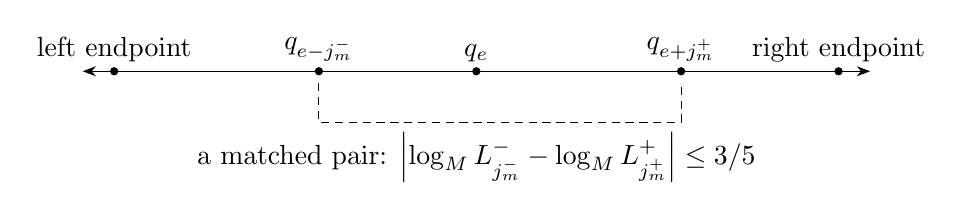
\begin{tikzpicture}[x=1cm,y=1cm,>=Stealth]
  \draw[->] (0,0)--(-5,0);
  \draw[->] (0,0)--(5,0);
  \foreach \x in {-4.6,-2,0,2.6,4.6}
    \fill (\x,0) circle (1.5pt);
  \node[above] at (0,0) {$q_e$};
  \node[above] at (-2,0) {$q_{e-j_m^-}$};
  \node[above] at (2.6,0) {$q_{e+j_m^+}$};
  \node[above] at (-4.6,0) {left endpoint};
  \node[above] at (4.6,0) {right endpoint};
  \draw[densely dashed] (-2,-.15)--(-2,-.65)--(2.6,-.65)--(2.6,-.15);
  \node[below,align=center] at (0,-.65)
    {a matched pair: $\abs{\log_M L_{j_m^-}^- -\log_M L_{j_m^+}^+}\le3/5$};
\end{tikzpicture}
\caption{The two paths are followed outward from a fixed central position.
Matched indices need not be equally far from the center; their derivatives
with respect to the other central coordinate have comparable logarithmic
size.}
\label{can:wing-figure}
\end{figure}

\subsection{The local input}

The analytic fact used at each matched pair is the following uniform
scarcity statement.  Its proof occupies \cref{loc:section}.

\begin{lemma}[Local scarcity]\label{can:local-scarcity}
For every $\eta>0$ there are $\eta'>0$ and $M_\eta<\infty$ such that
the following holds for $M\ge M_\eta$.  Fix $q_e$, a base coordinate
$\theta_*$, and indices $j_+,j_-\ge2$ on the two outward paths.
Suppose both indices are good at $\theta_*$ for a common normalized
solution, and their logarithms satisfy
\cref{can:matching-condition}.  Let
\[
L_+=\abs{t_{j_+}^+(\theta_*)},\qquad
L_-=\abs{t_{j_-}^-(\theta_*)},\qquad L=\max(L_+,L_-).
\]
Let $\mathcal S\subset[-1,1]$ consist of the $h$ for which, at
$\theta=\theta_*+h/L$, the same two indices are good for some common
solution with $u_e=1$.  The solution is allowed to depend on $h$, and
neither endpoint smallness nor a new matching condition is required at
these other points.  Then
\begin{equation}\label{can:scarcity-bound}
\abs{\{x\in\R:\dist(x,\mathcal S)<\eta'\}}\le\eta.
\end{equation}
Here and below the size of a subset of the line or circle denotes its
Lebesgue measure.  The constants are uniform over the central position,
the base coordinate, and the selected indices.
\end{lemma}

\subsection{From local scarcity to exponential decay}

\begin{proof}[Proof of \cref{can:theorem}]
Fix once and for all a sufficiently small $\delta>0$ allowed by
\cref{can:matching}.  Its constants $c_1,C_1,n_*$ are now fixed.
Choose $\eta>0$ so small that
\begin{equation}\label{can:eta-choice}
5\eta<1,\qquad
c_1\log\frac1{5\eta}>C_1+1.
\end{equation}
Obtain $\eta'$ and $M_\eta$ from \cref{can:local-scarcity}.  Increase
a fixed lower bound $M_0$ so that all estimates above hold, that
$M_0\ge M_\eta$, and that
\begin{equation}\label{can:radius-choice}
M_0^{-c}<\frac14,\qquad M_0^{-c}/5<\eta'.
\end{equation}
These choices are independent of $n$, of the center, and of $M\ge M_0$.

Fix $e\in\{0,-1\}$ and $q_e$.  It is enough to consider patterns
containing exactly $r=\lceil c_1n\rceil$ pairs, since a longer pattern
can be truncated.  For a fixed such increasing pattern, let
$\mathcal F$ be the set of $\theta$ admitting one common normalized
solution with all of the following properties: the original central
pair has norm at most $\sqrt2$; both endpoint pairs satisfy
\cref{can:small-solution}; and every pair of selected indices is good
and satisfies \cref{can:matching-condition}.  We emphasize that one
solution must satisfy all conditions of a pattern at once.

The set $\mathcal F$ is measurable, in fact compact.  To see this without
selecting solutions, parameterize the original central pair by its entry
other than the fixed entry $u_e=1$.  The norm bound puts that parameter in
$[-1,1]$.  All later solution entries and all recurrence coefficients
depend continuously on this parameter and on the circle coordinate
$\theta$.  Each pair entering a logarithm is nonzero, by invertibility
of the recurrence.  The endpoint, goodness, and matching conditions are
closed inequalities on the compact product of the circle with
$[-1,1]$.  Their projection is therefore compact.

For $\theta\in\mathcal F$ and $1\le m\le r$, define
\[
L_m(\theta)=\max\left(
\abs{t_{j_m^+}^+(\theta)},\abs{t_{j_m^-}^-(\theta)}\right),
\qquad s_m(\theta)=L_m(\theta)^{-1},
\]
and let
\[
V_m=\bigcup_{\theta\in\mathcal F}
 B\bigl(\theta,s_m(\theta)/10\bigr)
\]
be an open subset of the circle.  Goodness at the later of two selected
indices gives, separately on both paths,
\[
\abs{t_{j_{m+1}^\pm}^\pm(\theta)}
\ge M^{c(j_{m+1}^\pm-j_m^\pm)}
      \abs{t_{j_m^\pm}^\pm(\theta)}.
\]
Since both index sequences increase strictly,
\begin{equation}\label{can:radius-decay}
s_{m+1}(\theta)\le M^{-c}s_m(\theta),
\qquad s_m(\theta)\le M^{-c}.
\end{equation}
For fixed $M,n$, these positive radii also have a positive lower bound:
the one-step norm bound gives $\abs{t_j}\le M^{j-1}\le M^n$ at all
indices in question, so $s_m\ge M^{-n}$.

We claim
\begin{equation}\label{can:cover-contraction}
\abs{V_{m+1}}\le5\eta\abs{V_m}\qquad(1\le m<r).
\end{equation}
Select disjoint balls from the family defining $V_m$ as follows.  At each
stage select a remaining ball whose radius is at least half the
supremum of the remaining radii, and remove all remaining balls meeting
it.  Assign each removed ball to this selected ball.  All selected balls
are disjoint and have a fixed positive lower radius, so only finitely
many can be selected on the circle; the procedure must exhaust the
family.  Every assigned ball meets its selected ball and has radius at
most twice that of the selected ball.

Consider one selected center $\theta_*$ and write
$s=s_m(\theta_*)$.  The centers of its assigned balls are at circle
distance at most $3s/10$ from $\theta_*$.  The window of radius $s$ is
an injective lift interval by \cref{can:radius-choice,can:radius-decay}.
All assigned centers belong to $\mathcal F$, so they are successful for
the same selected pair of indices in the local test based at
$\theta_*$.  A next-level ball centered at an assigned $\theta$ has
radius at most
\[
\frac{s_{m+1}(\theta)}{10}
\le \frac{M^{-c}s_m(\theta)}{10}
\le \frac{M^{-c}s}{5}.
\]
After rescaling the lifted coordinate by $1/s$, the union of all these
next-level balls is contained in the $\eta'$-neighborhood of the
successful set in \cref{can:local-scarcity}, by
\cref{can:radius-choice}.  It therefore has unscaled length at most
$\eta s$.  Summing over selected balls proves
\[
\abs{V_{m+1}}\le\eta\sum_{\text{selected}}s
=5\eta\sum_{\text{selected}}
  \abs{B(\theta_*,s/10)}
\le5\eta\abs{V_m},
\]
as claimed.  The ball selected at a center is included in its own
assigned group, so no next-level balls have been omitted.

Since $\mathcal F\subset V_m$ for every $m$ and $\abs{V_1}\le1$,
iteration gives
\[
\abs{\mathcal F}\le(5\eta)^{r-1}
\le(5\eta)^{-1}
  \exp\left(-c_1n\log\frac1{5\eta}\right).
\]
There are at most $\exp(C_1n)$ patterns.  By
\cref{can:eta-choice}, their union has circle measure at most
$C\exp(-\gamma n)$ for a fixed $\gamma>0$, uniformly in the fixed
coordinate $q_e$.  The coordinate pair $(q_e,q_{e-1})$ has normalized
product Lebesgue law.  Integrating the conditional bound over $q_e$ and
summing the two choices of $e$ therefore gives the same form of bound
for the original event, for every $n\ge n_*$.  Every point of that event
is covered, by \cref{can:small-solution,can:matching}.  Finally enlarge
$C$ to cover the finitely many positive integers $n<n_*$, whose event
probabilities are at most one.  Stationarity restores every center $i$.
\end{proof}

\section{Local scarcity at matched scales}
\label{loc:section}

This section proves \cref{can:local-scarcity}. We use its two outward
paths and the notation established in the cancellation argument. In
particular, $c=99/100$, the central coordinate is fixed, and the variable
is $\theta=q_{e-1}$. The selected indices are denoted by $j_+$ and
$j_-$. Every assertion concerning an interval in $\theta$ uses real
lifts of the recurrence. The constants below are independent of the
selected indices and of the base configuration.

The central relation in \cref{can:center-equation} will become, after rescaling, an approximate
identity between a cubic polynomial and two shifted reciprocal-cosine
terms. A positive-measure Hausdorff limit of the closures of successful
sets would force an analytic identity. We rule out that identity even when the two
reciprocal terms nearly cancel or one phase slope tends to zero. The
derivative estimates in the first two subsections provide the uniform
remainders needed for these two degeneracies.

\subsection{Control on a single rescaled path}

Fix either outward path and write $j$ for its selected index. Put
\[
 L_j=\abs{t_j(\theta_*)},\qquad
 \xi=L_j(\theta-\theta_*),\qquad D=\frac{\dd}{\dd\xi}.
\]
The initial position $q_0$ is constant and $q_1$ is affine in $\xi$,
with derivative $\pm L_j^{-1}$. By \cref{can:good-t}, the base
linearized solution satisfies
\begin{equation}
 \frac{\abs{t_l(\theta_*)}}{L_j}
 \le M^{-c(j-l)}\quad(1\le l\le j).
 \label{loc:base-growth}
\end{equation}
We will prove, throughout $\abs{\xi}\le1$, that
\begin{align}
 \abs{q_l(\xi)-q_l(0)}+\abs{Dq_l(\xi)}
 &\le C M^{-c(j-l)}, \label{loc:first-derivatives}\\
 \abs{D^p q_l(\xi)}
 &\le C_p M^{-pc(j-l)}M^{1-pc}
 \quad(2\le p\le5), \label{loc:higher-derivatives}
\end{align}
for $0\le l\le j$. The terms with $l=0$ vanish.

Write $B_l=M^{-c(j-l)}$ and $\Delta_l=q_l(\xi)-q_l(0)$.
Taylor's formula for the recurrence, followed by propagation with the
base linearized matrices, gives
\begin{equation}
 \abs{\Delta_l}
 \le \abs{\xi}\frac{\abs{t_l(\theta_*)}}{L_j}
       +C\sum_{d=1}^{l-1}M^{l-d}\abs{\Delta_d}^2.
 \label{loc:nonlinear-comparison}
\end{equation}
Here the quadratic error at site $d$ is at most $CM\abs{\Delta_d}^2$,
and the remaining $l-d-1$ steps have norm at most $M^{l-d-1}$.
For $l=1$ the estimate $\abs{\Delta_l}\le2B_l$ follows directly
from \cref{loc:base-growth}. If it holds for all earlier indices,
the sum in \cref{loc:nonlinear-comparison} is bounded by
\[
 4C B_l^2\sum_{a\ge1}M^{(1-2c)a}.
\]
Since $B_l\le1$ and $1-2c<0$, this is at most $B_l$ for all
sufficiently large $M$. Induction proves the required displacement
bound, uniformly in $j$.

Compare $Dq_l(\xi)$ with the base variation
$\pm t_l(\theta_*)/L_j$. Their initial data agree. Their difference
is propagated by the base matrices with forcing
\[
 \bigl(v(q_d(\xi))-v(q_d(0))\bigr)Dq_d(\xi),
\]
whose absolute value is at most $CM\abs{\Delta_d}\abs{Dq_d}$.
Induction with $\abs{Dq_d}\le2B_d$ therefore uses the same geometric
sum and proves \cref{loc:first-derivatives}.

For completeness, the higher derivative induction uses the recurrence
at the varied orbit. For $p\ge2$ it has the form
\[
 D^p q_{l+1}=v(q_l)D^p q_l-D^p q_{l-1}+F_{p,l},
\]
where $F_{p,l}$ is a finite sum, with coefficients depending only on
$p$, of terms
\[
 \phi^{(s)}(q_l)\prod_{i=1}^{s}D^{m_i}q_l,
 \qquad 2\le s\le p,\quad m_i\ge1,\quad
 \sum_{i=1}^{s}m_i=p.
\]
Each $m_i$ is strictly smaller than $p$. The first derivative bound
and the induction hypothesis give
$\abs{D^{m_i}q_l}\le C_{m_i}B_l^{m_i}$, since
$M^{1-m_ic}\le1$ whenever $m_i\ge2$. Consequently
$\abs{F_{p,l}}\le C_p M B_l^p$. The initial higher derivatives
at sites $0,1$ vanish. Propagation by the varied matrices gives
\[
 \abs{D^p q_l}
 \le C_p\sum_{d=1}^{l-1}M^{l-d}B_d^p
 \le C_p B_l^p\sum_{a\ge1}M^{(1-pc)a}
 \le C'_p B_l^p M^{1-pc}.
\]
This proves \cref{loc:higher-derivatives} successively for
$p=2,3,4,5$.

At the selected site $Dq_j(0)=\pm1$. The case $p=2$ shows that
\[
 Dq_j(\xi)=Dq_j(0)+O(M^{1-2c}).
\]
It follows, for all sufficiently large $M$, that
\begin{equation}
 \abs{t_j(\xi)}\ge L_j/2,\qquad
 \abs{t_l(\xi)}\le C L_j M^{-c(j-l)}\quad(l<j).
 \label{loc:varied-t}
\end{equation}
The quotient
\begin{equation}
 E=\frac{t_{j-1}}{t_j}=\frac{Dq_{j-1}}{Dq_j}
 \quad\hbox{satisfies}\quad
 \abs{D^p E}\le C_p M^{-c}\quad(0\le p\le4).
 \label{loc:quotient}
\end{equation}
Indeed the denominator is bounded away from zero. Every derivative of
its reciprocal of order at most four is bounded by the already proved
bounds through $D^5q_j$. Every derivative of the numerator through
order four contains a derivative of $q_{j-1}$ and has a factor at most
$CM^{-c}$. The product rule proves \cref{loc:quotient}.

\subsection{A fourth derivative bound for the boundary value}

Fourth-order control makes the boundary value replaceable by a cubic
polynomial with a small remainder. The remainder must remain negligible
even after normalizing the first nonzero correction when the two
reciprocal-cosine terms nearly cancel.

Let $R_j$ be the initial value at site $1$ of the solution $U$ with
$U_0=1$ and $U_j=0$. This solution exists throughout our interval
because $t_j$ does not vanish. We claim that, with $\rho=4/5$,
\begin{equation}
 L_j^2\abs{D^4R_j}\le C M^{-2-\rho}.
 \label{loc:boundary-fourth}
\end{equation}

Consider the $(j-1)$-by-$(j-1)$ tridiagonal matrix $B$ with diagonal
$v(q_a)$, $1\le a\le j-1$, and both adjacent diagonals equal to
$-1$. Its determinant is $t_j$: expansion along the last row gives
the same recursion and initial conditions as those for $t$.
The interior boundary problem is $BU=e_1$, so $R_j=(B^{-1})_{11}$.
More explicitly, its inverse $G=B^{-1}$ is
\begin{equation}
 G_{ab}=t_{\min(a,b)}U_{\max(a,b)}.
 \label{loc:green}
\end{equation}
To check this formula, fix column $b$. Its entries solve the homogeneous
recurrence except at row $b$, and are zero at the boundary sites $0,j$.
At row $b$ the output of $B$ is
$t_{b+1}U_b-t_bU_{b+1}=1$, by the constant Wronskian and the data
$t_0=0,t_1=1,U_0=1$. Thus the column is precisely $B^{-1}e_b$.

At the right boundary the same Wronskian gives
$U_{j-1}=1/t_j$. Backward propagation and
\cref{loc:varied-t} yield
\begin{equation}
 L_j\abs{U_a}\le2M^{j-a-1}.
 \label{loc:boundary-backwards}
\end{equation}
For $d_a=j-a\ge1$, \cref{loc:green,loc:varied-t,loc:boundary-backwards}
therefore give
\begin{equation}
 \abs{G_{ab}}\le C
 M^{\min(d_a,d_b)-1-c\max(d_a,d_b)}.
 \label{loc:green-size}
\end{equation}
The chain rule and the bounds for derivatives of $q_a$ also give
\begin{equation}
 \abs{D^p v(q_a)}\le C_p M^{1-cp d_a}
 \quad(1\le p\le4).
 \label{loc:potential-derivatives}
\end{equation}
In fact every term contains a derivative of $v$ bounded by $C_pM$
and derivatives of $q_a$ whose total order is $p$.

Starting with $DG=-G(DB)G$, differentiate three more times and take
the $(1,1)$ entry. The result is a finite linear combination, with
fixed integer coefficients, of sums of terms
\begin{equation}
 U_{a_1}(D^{p_1}v_{a_1})G_{a_1a_2}
 (D^{p_2}v_{a_2})\cdots
 G_{a_{s-1}a_s}(D^{p_s}v_{a_s})U_{a_s},
 \qquad p_i\ge1,\quad \sum_{i=1}^{s}p_i=4.
 \label{loc:inverse-chains}
\end{equation}
Here $v_a=v(q_a)$, $1\le s\le4$, and each site index is summed
independently from $1$ to $j-1$. This form follows inductively:
differentiating a potential factor increases its derivative order,
whereas differentiating any inverse factor inserts another
$-G(DB)G$. Also $G_{1a}=U_a$ because $t_1=1$.

Put $d_i=j-a_i$. After multiplication by $L_j^2$, the exponent of
$M$ bounding a term of \cref{loc:inverse-chains} is
\begin{align*}
 H&=-1+d_1+d_s+
 \sum_{i=1}^{s-1}\bigl(\min(d_i,d_{i+1})-c\max(d_i,d_{i+1})\bigr)
       -c\sum_{i=1}^{s}p_id_i\\
 &\le -1+2\min_i d_i-(3c-2)\sum_{i=1}^{s}p_id_i\\
 &\le -1-\frac{47}{100}\sum_{i=1}^{s}p_id_i.
\end{align*}
For the first inequality, write each adjacency term as
$-\abs{d_i-d_{i+1}}+(1-c)\max(d_i,d_{i+1})$. The total variation
is at least $d_1+d_s-2\min_i d_i$, while the sum of maxima is at
most $2\sum_i d_i\le2\sum_i p_id_i$. For the last inequality use
$4\min_i d_i\le\sum_i p_id_i$ and $c=99/100$.
Summing over sites is harmless: for every composition of $4$,
\[
 \sum_{d_1,\ldots,d_s\ge1}
 M^{-1-(47/100)\sum_i p_id_i}
 =M^{-1}\prod_{i=1}^{s}
 \frac{M^{-(47/100)p_i}}{1-M^{-(47/100)p_i}}
 \le C M^{-72/25}.
\]
There are only finitely many such compositions and chain types.
Since $72/25>2+4/5$, this proves \cref{loc:boundary-fourth}.

\subsection{The cubic relation at successful points}

Return to the two paths and put
$L=\max(L_{j_+},L_{j_-})$, $h=L(\theta-\theta_*)$.
Number the paths so that the first has the larger base scale. Write
$Q_i(h)$ for their selected positions and $E_i(h)$ for the quotients
in \cref{loc:quotient}. With $b_i=Q_i'(0)$ and $d_i=Q_i''(0)$,
the preceding estimates imply
\begin{align}
 Q_i(h)&=z_i+b_ih+\tfrac12d_ih^2+\mathcal E_i(h),
 &\norm{\mathcal E_i}_{C^1([-1,1])}
   &\le C\abs{b_i}^3M^{1-3c}, \label{loc:phase-taylor}\\
 \abs{d_i}&\le C\abs{b_i}^2M^{1-2c},
 &\abs{b_1}&=1,\quad
 \abs{b_2}=r\in[M^{-3/5},1], \label{loc:phase-slopes}\\
 \abs{\partial_h^pE_i}&\le C_pM^{-c}\abs{b_i}^p
 &&(0\le p\le4). \label{loc:scaled-quotient}
\end{align}
The scale change is $\xi=(L_{j_i}/L)h=\abs{b_i}h$.
It also gives, for $2\le p\le5$,
\begin{equation}
 \abs{Q_i^{(p)}}\le C_p\abs{b_i}^pM^{1-pc},\qquad
 \abs{Q_i'}\asymp\abs{b_i}.
 \label{loc:scaled-phase-derivatives}
\end{equation}

At a successful point there is a common solution with central value
$1$, and its two outward values at site $1$ add to $v(q_e)$.
Apply \cref{can:boundary-expansion} to both paths at that point.
Since $\abs{t_{j_i}(\theta)}=L\abs{Q_i'(h)}$ and
$v(Q_i)-E_i=K(\cos(2\pi Q_i)+(2-E_i)/K)$, multiplication by
$KL^2$ yields
\[
 KL^2\left(v(q_e)-\sum_{i=1}^{2}R_{j_i}(\theta)\right)
 =\sum_{i=1}^{2}
 \frac{1}{(Q_i')^2(\cos(2\pi Q_i)+(2-E_i)/K)}
 +O(r^{-2}M^{1-3c}).
\]
The error bound uses \cref{loc:scaled-phase-derivatives} to compare
the varied $t_{j_i}$ with their base sizes. Replace the left side by
its cubic Taylor polynomial $P(h)$ at $0$. The contribution of each
$R_{j_i}$ to the Taylor remainder is at most
\[
 C K L^2\abs{b_i}^4 L_{j_i}^{-2}M^{-2-\rho}
 =C K\abs{b_i}^2M^{-2-\rho}.
\]
Consequently every successful $h\in[-1,1]$ satisfies
\begin{equation}
 P(h)=\sum_{i=1}^{2}
 \frac{1}{(Q_i'(h))^2
       (\cos(2\pi Q_i(h))+(2-E_i(h))/K)}
       +O(M^{-1-\rho}+r^{-2}M^{1-3c}).
 \label{loc:cubic-relation}
\end{equation}
The polynomial may depend on the configuration. Its degree is at
most three. The displayed error is uniform on the successful set,
and tends to zero uniformly over all configurations, since
$r^{-2}M^{1-3c}\le M^{-77/100}$.

\subsection{Polynomial extraction from a Hausdorff limit}

Consider any sequence of configurations with $M\to\infty$ and
nonempty successful sets $\mathcal S_M$. Pass to a subsequence on
which their closures converge in Hausdorff distance to a nonempty
compact set $F\subset[-1,1]$. We prove that $F$ has measure zero.
Suppose to the contrary that it has positive measure.

We record precisely the compactness argument for the polynomials
that will be used below. Suppose, after an indicated subtraction
or multiplication of \cref{loc:cubic-relation}, a polynomial $P_M^*$
of degree at most three agrees at successful points, up to an error
tending to zero, with functions converging uniformly on every compact
subinterval of $[-1,1]$ away from a fixed finite set of limiting poles
in that interval. Choose four
distinct points of $F$ outside those poles. Hausdorff convergence
and approximation of points in the closure supply successful points
converging to these four points. The values of $P_M^*$ there are
bounded. The associated Vandermonde matrices converge to an invertible
matrix, so all four coefficients of $P_M^*$ are bounded. Pass to a
further subsequence on which the polynomials converge coefficientwise.
For every point of $F$ away from the poles the same approximation
argument shows equality with the limiting function. In particular,
equality holds on a set of positive measure. Clearing the finitely
many denominator factors used in that case gives an identity between
real analytic functions on $\R$: the difference has an accumulation
point of zeros and hence vanishes identically. Passing to further
subsequences throughout does not change the fixed Hausdorff limit $F$.

\subsection{Nonzero limiting slopes and opposite cosines}

First suppose that $r$ has a positive limit $r_0$. Take convergent
subsequences of the phases modulo integers and of the slopes. The
first slope has a fixed sign after a further subsequence, so write
its value as $b\in\{-1,1\}$. By
\cref{loc:phase-taylor,loc:scaled-quotient}, the two terms on the
right of \cref{loc:cubic-relation} converge, away from their limiting
poles, to
\[
 \sec(2\pi(z+bh))+
 r_0^{-2}\sec(2\pi(z'+b'h)),\qquad \abs{b'}=r_0.
\]
Polynomial extraction and multiplication by both cosines show that
the zero sets of these cosines on $\R$ coincide: at a zero of either
cosine, the other must vanish because its coefficient is positive.
Their zero sets are arithmetic progressions with respective spacings
$1/(2\abs{b})$ and $1/(2\abs{b'})$, so $r_0=1$.
The two cosines are therefore equal or opposite. Equality would leave
twice a secant, which cannot equal a polynomial, as multiplication by
the cosine and evaluation at one of its zeros shows. Only the opposite
case remains.

Reflect the second phase if necessary and translate it by an odd
half-integer. The resulting phase $\widetilde Q_2$ has the same
limiting affine phase as $Q_1$, while
\[
 \cos(2\pi Q_2)=-\cos(2\pi\widetilde Q_2),\qquad
 (Q_2')^2=(\widetilde Q_2')^2.
\]
By \cref{loc:phase-taylor},
\begin{equation}
 \widetilde Q_2-Q_1=p(h)+O_{C^1}(M^{1-3c}),\qquad
 \deg p\le2,\qquad \norm{p}_{\rm coeff}\longrightarrow0.
 \label{loc:phase-difference}
\end{equation}
Here $\norm{p}_{\rm coeff}$ is the maximum absolute value of its
three coefficients. Define
\[
 \ell=\max(\norm{p}_{\rm coeff},K^{-1}).
\]
Then $\ell\to0$, but every error of order $M^{1-3c}=M^{-197/100}$
is $o(\ell)$. The error in \cref{loc:cubic-relation} is also
$o(\ell)$ in the present case, since $r\to1$ and $\rho>0$.

We expand on a compact subinterval away from the zeros of the common
limiting cosine. Put
\[
 f(x,y)=y^{-2}\sec(2\pi x),\qquad
 A=2\pi(z_1+b_1h).
\]
The denominators in \cref{loc:cubic-relation} stay uniformly away
from zero there for large $M$. Their shifts are
$2/K+O(M^{-c}/K)$. Expanding the reciprocals, with their respective
cosine signs, gives the sum of the two terms as
\begin{align*}
 &f(Q_1,Q_1')-f(\widetilde Q_2,\widetilde Q_2')\\
 &\quad-\frac2K\left((Q_1')^{-2}\sec^2(2\pi Q_1)
            +(\widetilde Q_2')^{-2}\sec^2(2\pi\widetilde Q_2)\right)
       +o(\ell).
\end{align*}
The reciprocal expansion has error $O(K^{-2}+M^{-c}/K)=o(\ell)$.
It is essential to subtract the two $f$ terms at the actual common
phase before replacing that phase by an affine one. Taylor expansion
of $f$, using \cref{loc:phase-difference}, gives
\[
 f(Q_1,Q_1')-f(\widetilde Q_2,\widetilde Q_2')
 =-f_x(Q_1,Q_1')p-f_y(Q_1,Q_1')p'+o(\ell).
\]
Indeed the quadratic error is $O(\ell^2)$ and the phase remainder
is $O(M^{1-3c})$. Moreover
$(Q_1,Q_1')=(z_1+b_1h,b_1)+O(M^{1-2c})$; replacing the derivatives
of $f$ by their values at this affine pair produces only
$O(\ell M^{1-2c})=o(\ell)$. Similarly, the preceding $K^{-1}$ term
can be evaluated at the common affine pair with error $o(K^{-1})$.
We conclude that \cref{loc:cubic-relation} becomes
\begin{equation}
 P(h)=\frac{2p'}{b_1^3}\sec A
      -\frac{2\pi p}{b_1^2}\sin A\,\sec^2 A
      -\frac4{K b_1^2}\sec^2 A+o(\ell).
 \label{loc:opposite-expansion}
\end{equation}

Divide by $\ell$ and take a subsequence such that
$p/\ell\to\bar p$ coefficientwise and $K^{-1}/\ell\to\beta$.
At least one is nonzero, because
$\max(\norm{p/\ell}_{\rm coeff},K^{-1}/\ell)=1$.
Polynomial extraction now applies to $P/\ell$. Multiply its limiting
identity by $b^2\cos^2(2\pi(z+bh))$ and evaluate at every zero of
that cosine. One obtains
\begin{equation}
 2\pi\bar p(h)\sin(2\pi(z+bh))+4\beta=0
 \quad\hbox{at every cosine zero.}
 \label{loc:alternating-obstruction}
\end{equation}
The zeros form an unbounded arithmetic progression and their sine
values alternate between $1$ and $-1$. Thus $\bar p$ is bounded on
that progression and must be constant. The alternating signs then
force both that constant and $\beta$ to be zero, contradicting their
normalization. This excludes every positive limiting slope.

\subsection{A vanishing second slope}

It remains to treat $r\to0$. After a subsequence, the first term of
\cref{loc:cubic-relation} converges away from its poles to
$\sec(2\pi(z+bh))$, with $\abs{b}=1$. Write the second term as
\begin{equation}
 g(h)=\frac1{r^2S(h)},\qquad
 S(h)=\left(\frac{Q_2'(h)}r\right)^2
       \left(\cos(2\pi Q_2(h))+\frac{2-E_2(h)}K\right),
 \qquad w=\max(\abs{S(0)},r).
 \label{loc:slow-denominator}
\end{equation}
Uniformly on $[-1,1]$,
\begin{equation}
 \abs{S^{(m)}}\le C_m r^m\quad(1\le m\le4).
 \label{loc:slow-derivatives}
\end{equation}
To see every derivative involved, set $a=Q_2'/r$. Then $a$ is
bounded and bounded away from zero, and
\[
 \abs{a^{(m)}}\le C_m r^m M^{1-(m+1)c}\le C_m r^m
 \quad(1\le m\le4)
\]
by \cref{loc:scaled-phase-derivatives}. The derivatives through
order four of the cosine factor are $O(r^m)$ by the chain rule;
those of the shift are bounded by $C_mr^mM^{-c}/K$ by
\cref{loc:scaled-quotient}. The product rule proves
\cref{loc:slow-derivatives}. This is the point requiring the fifth
derivative of $Q_2$.

If $w\to0$, there is also the sharper fact
\begin{equation}
 \frac{\abs{S'(0)}}r\longrightarrow2\pi.
 \label{loc:slow-nonzero-slope}
\end{equation}
Indeed $a(0)^2=1$ and $\abs{Q_2'(0)}=r$. The cosine with its shift
equals $S(0)\to0$, so $\abs{\sin(2\pi Q_2(0))}\to1$.
Differentiating the factor $a^2$ contributes
$O(rwM^{1-2c})=o(r)$; differentiating the shift contributes
$O(rM^{-c}/K)=o(r)$. The remaining contribution is
$-2\pi\sin(2\pi Q_2(0))Q_2'(0)$, which proves the assertion.

Take a subsequence on which $r/w$ has a limit. If this limit is
positive, then $w\to0$, and Taylor's formula gives
\[
 \frac{S(h)}w=\frac{S(0)}w+\frac{S'(0)}w h+O(r^2/w).
\]
Here $r^2/w\le r\to0$. The coefficients are bounded; by
\cref{loc:slow-nonzero-slope}, a further subsequence gives a limiting
affine polynomial $A_0(h)$ with nonzero slope. Multiply
\cref{loc:cubic-relation} by $r^2w$. Its first term and its error
tend to zero locally away from the fast poles, while its second term
converges to $1/A_0(h)$ away from the one possible zero of $A_0$.
Polynomial extraction would therefore give a polynomial of degree
at most three equal to $1/A_0$. Multiplication by $A_0$ and evaluation
at its real zero is a contradiction.

We may consequently assume $r/w\to0$. Then $w=\abs{S(0)}$
eventually, and
\begin{equation}
 \frac{S(h)}{S(0)}=1+O(r/w)\longrightarrow1
 \quad\hbox{uniformly on }[-1,1].
 \label{loc:almost-constant-denominator}
\end{equation}
In particular $S$ has no zeros there for large $M$.
Let $T_3g$ be the cubic Taylor polynomial of $g$ at $0$.
If $w$ stays bounded away from zero, the reciprocal derivative formula
and \cref{loc:slow-derivatives} give $g^{(4)}=O(r^2)$ uniformly.
Thus $g-T_3g=O(r^2)$. Subtracting $T_3g$ from
\cref{loc:cubic-relation} leaves only the fast secant in the limit.
It cannot agree with a cubic polynomial, by multiplication by its
cosine and evaluation at a zero.

The last case is $w\to0$ and $r/w\to0$. To track also the possibly
large remainder of $g$, differentiate explicitly:
\begin{equation}
 g^{(4)}=\frac1{r^2}\left(
 \frac{24(S')^4}{S^5}
 -\frac{36(S')^2S''}{S^4}
 +\frac{6(S'')^2+8S'S'''}{S^3}
 -\frac{S''''}{S^2}\right).
 \label{loc:reciprocal-fourth}
\end{equation}
By \cref{loc:slow-derivatives,loc:slow-nonzero-slope},
$S'(h)/S'(0)=1+O(r)$ uniformly. Together with
\cref{loc:almost-constant-denominator}, this makes the first term
in \cref{loc:reciprocal-fourth} equal to
\[
 (24+o(1))\frac{S'(0)^4}{r^2S(0)^5}.
\]
Relative to that term, the remaining three displayed contributions
are respectively $O(w)$, $O(w^2)$, and $O(w^3)$: for example the
first ratio is bounded by $C\abs{S}\abs{S''}/\abs{S'}^2\le Cw$.
All these comparisons are uniform on $[-1,1]$. Put
\[
 a_M=\frac{S'(0)^4}{r^2S(0)^5}.
\]
Taylor's formula with integral remainder, valid on both sides of
zero, now yields
\begin{equation}
 g(h)-T_3g(h)=a_Mh^4+o(\abs{a_M})
 \quad\hbox{uniformly on }[-1,1].
 \label{loc:quartic-remainder}
\end{equation}
If $\abs{a_M}\to\infty$, subtract $T_3g$ from
\cref{loc:cubic-relation} and divide by $a_M$. The fast term tends
to zero away from its poles and the original error also tends to
zero after this division. Polynomial extraction would identify a
polynomial of degree at most three with $h^4$, which is impossible.
Otherwise pass to a subsequence with $a_M\to a\in\R$.
Without division, the same subtraction gives a limiting identity
between a cubic polynomial and
\[
 \sec(2\pi(z+bh))+ah^4.
\]
Move the quartic term to the polynomial side and multiply by the
cosine. Evaluation at any of its zeros again gives a contradiction.
These alternatives exhaust the vanishing-slope case.

\subsection{Uniform neighborhoods of successful sets}

We have proved that every Hausdorff limit of nonempty closures of
successful sets along $M\to\infty$ has measure zero. This implies
the uniform assertion of \cref{can:local-scarcity}, including the
neighborhood width in its statement. Indeed, if the assertion failed
for some $\eta>0$, then for every integer $n$ one could choose
$M_n\ge n$ and a successful set $\mathcal S_n\subset[-1,1]$ such
that
\[
 \operatorname{Leb}_{\R}\{x:\dist(x,\mathcal S_n)<1/n\}>\eta.
\]
These sets are nonempty. Compactness of the nonempty compact subsets
of $[-1,1]$ for Hausdorff distance supplies a subsequence of their
closures with limit $F$. For every $\varepsilon>0$, eventually
\[
 \{x:\dist(x,\mathcal S_n)<1/n\}
 \subset\{x:\dist(x,F)<\varepsilon\}.
\]
Thus every $\varepsilon$-neighborhood of $F$ has measure at least
$\eta$. Continuity of Lebesgue measure from above for these bounded
neighborhoods implies $\operatorname{Leb}_{\R}(F)\ge\eta$,
contrary to the result just proved. The empty successful set satisfies
the claimed estimate automatically. This completes the proof of
\cref{can:local-scarcity}.

\section{A product estimate across a fast bridge}
\label{bridge:section}

The second estimate compares observations near opposite ends of a long
interval on which the transfer matrix grows almost at its maximum rate.
The comparison comes from two transverse families of contracting graphs
in the middle of the interval. All measures in this section are the
normalized area measure, expressed in the coordinates
$(q_i,q_{i-1})$ when convenient, whenever they define probabilities
or expectations. Label lengths and slice integrals use ordinary
one-dimensional Lebesgue measure in their displayed coordinates.

For distinct integers $d,e$, write
\begin{equation}
 \mathfrak h_{d,e}
   =1-\frac{\log_M\norm{T_{d,e}}}{\abs{d-e}}.
 \label{bridge:shortfalls}
\end{equation}
These quantities belong to $[0,1]$. An observation with bound $(R,L,B)$
means a function of at most $R$ such quantities whose defining function
on $[0,1]^R$ has absolute value at most $B$ and Lipschitz constant at most
$L$ for the maximum norm. Allowing fewer than $R$ arguments is harmless.
The defining functions and the integer indices may vary from one
application to another, provided these bounds are preserved.
Equivalently, these bounds may be imposed only on the realized range
$\mathcal R\subseteq[0,1]^R$ of the arguments. Indeed, a function $f$
on that range extends by
$u\mapsto\inf_{v\in\mathcal R}(f(v)+L\norm{u-v}_\infty)$;
clipping this extension to $[-B,B]$ preserves its values on
$\mathcal R$ and its Lipschitz bound.

\begin{theorem}[Product estimate across a fast bridge]
\label{bridge:theorem}
There are absolute constants $c_b\in(0,1)$, $\kappa>0$, and $\sigma>0$
with the following property. Fix observation bounds $(R,L,B)$ and a
threshold $h>0$. For sufficiently large $M$ and sufficiently large
$n=b-a$, let $W,H$ be observations with these bounds, with $W\geq0$.
All indices occurring in one observation are within $\kappa n$ of $a$,
and all indices occurring in the other are within $\kappa n$ of $b$.
Either assignment of $W,H$ to the two ends is allowed. Then
\begin{equation}
 \E\!\left[
   \one_{\{\log_M\norm{T_{a,b}}\geq c_b n\}}
   W\one_{\{H>h\}}
 \right]
 \leq
 C\bigl(\E W+M^{-\sigma n}\bigr)\PP(H>h/2).
 \label{bridge:product}
\end{equation}
The constants $c_b,\kappa,\sigma$ are independent of the observation
bounds and threshold. The constant $C$ and the lower size requirements
for $M,n$ may depend on $(R,L,B)$ and $h$, but not on the indices,
the defining functions, or the bridge location.
\end{theorem}

We first construct the graphs needed in the proof. Finite-time
contracting directions and curves have been developed in stable-manifold
constructions under weak hyperbolicity hypotheses
\cite{HollandLuzzatto2006}. Here the graphs are
level sets of a distant orbit coordinate, obtained from finite
Dirichlet problems; we prove their extent and transverse distortion
directly. We use $c=0.98$ throughout the construction. A direction is
understood modulo sign.

\begin{lemma}[Contracting graphs and their distortion]
\label{bridge:graphs}
For sufficiently large $M$, suppose $B_+\geq2$ and, at a fixed state with central coordinates
$(x,y)=(q_0,q_{-1})$,
\begin{equation}
 D_l:=\norm{T_{0,l}}\geq M^{cl}
 \qquad(1\leq l\leq B_+).
 \label{bridge:prefix-growth}
\end{equation}
For at least one choice $j\in\{B_+-1,B_+\}$ there is a smooth graph
through this state, parametrized by $q_{-1}=y+r$, $\abs r\leq1/4$,
on which the lifted coordinate $q_j$ is fixed. On this graph,
\begin{equation}
 \abs{q_p(r)-q_p(0)}+
 \abs{\frac{\dd q_p(r)}{\dd r}}
 \leq C M^{-0.8(p+1)}
 \qquad(0\leq p<j).
 \label{bridge:graph-contraction}
\end{equation}
The corresponding endpoint pair at time $B_+$ changes by at most
$C M^{-0.8(B_+-1)}$. The partial derivative
$\partial q_j/\partial q_0$, with $q_{-1}$ held independent, is
nonzero throughout the graph, and the absolute values of this partial
derivative at any two points of the graph have a ratio between two
absolute positive constants.

For a fixed choice of $j$, one may require the closed eligibility
condition
\begin{equation}
 \abs{\partial q_j/\partial q_0}\geq D_{B_+}/3
 \quad\text{at the initial point}.
 \label{bridge:row-choice}
\end{equation}
The graphs depend continuously on eligible initial points. There is
an identical backward statement, with almost horizontal graphs in
$(x,y)$, obtained by using $(q_{-1},q_0)$ as the ordered initial pair.
\end{lemma}

\begin{proof}
Let $s_l$ be a most contracted unit input direction for $T_{0,l}$.
Since a single inverse step has norm at most $M$,
\[
 \norm{T_{0,l}s_{l+1}}\leq\frac{M}{D_{l+1}}.
\]
The projection onto the expanded input direction for $T_{0,l}$
therefore gives
\begin{equation}
 \abs{s_{l+1}\wedge s_l}\leq\frac{M}{D_lD_{l+1}}.
 \label{bridge:direction-step}
\end{equation}
The absolute sine between two unoriented lines satisfies the triangle
inequality. Summing \cref{bridge:direction-step}, and using
\cref{bridge:prefix-growth}, yields
\[
 \abs{s_{B_+}\wedge s_l}
 \leq C M^{1-c-2cl}
 \qquad(1\leq l\leq B_+).
\]
Resolve $s_{B_+}$ into the singular input directions for $T_{0,l}$.
Using $D_l\leq M^l$ as well as its lower bound gives
\begin{equation}
 \norm{T_{0,l}s_{B_+}}
 \leq M^{-cl}+C M^{l+1-c-2cl}
 \leq C M^{-0.94l}.
 \label{bridge:stable-prefix}
\end{equation}
The last inequality follows from
$1-c+(1-2c)l=0.02-0.96l\leq-0.94l$ for $l\geq1$.

The first component of an input vector becomes the second component
after one step. Thus \cref{bridge:stable-prefix} at $l=1$ shows that
$s_{B_+}$ is nearly vertical. Let $t$ solve the variational recurrence
with $t_{-1}=0$, $t_0=1$. Horizontal input has a projection bounded
away from zero onto the expanded input direction for $T_{0,B_+}$.
For large $M$, at least one of the two coordinates $t_{B_+}$ and
$t_{B_+-1}$ consequently has magnitude at least $D_{B_+}/3$.
Choose the corresponding $j$. This proves that the two closed choices
in \cref{bridge:row-choice} cover the states under consideration.

The row of $T_{0,B_+}$ selecting $q_j$ has norm at least
$\abs{t_j}\geq D_{B_+}/3$, and its value on $s_{B_+}$ has magnitude
at most $D_{B_+}^{-1}$. Its kernel direction therefore differs from
$s_{B_+}$ by $O(D_{B_+}^{-2})$. Normalize that direction so that its
second component is 1, and let $U$ denote its variational solution.
Then $U_{-1}=1$, $U_j=0$, and, for $0\leq p<j$,
\begin{equation}
 \abs{U_p}\leq C M^{-0.9(p+1)}.
 \label{bridge:linear-dirichlet}
\end{equation}
Indeed, apply \cref{bridge:stable-prefix} at $l=p+1$ to its main
component. The error component is bounded by
\[
 C M^{p+1}D_{B_+}^{-2}
 \leq C M^{-0.96(p+1)},
\]
because $p+1\leq B_+$. Normalization changes these bounds only by an
absolute factor.

We now solve the nonlinear boundary problem. Let $\xi_p$ be the
change of the lifted position $q_p$, with boundary data
$\xi_{-1}=r$ and $\xi_j=0$. The tridiagonal matrix on
$0,\ldots,j-1$ with diagonal $v(q_p)$ and adjacent entries $-1$
has determinant $t_j\ne0$. Its inverse is
\begin{equation}
 G_{lp}=t_{\min(l,p)}U_{\max(l,p)}.
 \label{bridge:green}
\end{equation}
For completeness, the proposed column solves the homogeneous
recurrence except at its source. At that source the output is 1,
because the Wronskian
$t_{p+1}U_p-t_pU_{p+1}$ equals its boundary value 1. Both boundary
values of the proposed column are zero. This verifies
\cref{bridge:green} directly.

Subtract the original orbit recurrence from the new one, and move
the nonlinear Taylor remainder to the right side. With its sign
absorbed into $F_p$, the boundary problem becomes
\begin{equation}
 \xi_l=U_l r+\sum_{p=0}^{j-1}G_{lp}F_p(\xi_p),
 \qquad
 \abs{F_p(u)}\leq C M u^2,
 \quad
 \abs{F'_p(u)}\leq C M\abs u.
 \label{bridge:fixed-point}
\end{equation}
Use the finite-dimensional weighted norm
\[
 \norm{\xi}_*=\max_{0\leq l<j}
          M^{0.8(l+1)}\abs{\xi_l}.
\]
On a ball of fixed radius $R_0$, the Lipschitz bound for the nonlinear
part of \cref{bridge:fixed-point}, before weighting its output at
index $l$, is bounded by a constant depending on $R_0$ times
\[
 \sum_{p\leq l}
 M^{p-0.9(l+1)+1-1.6(p+1)}
 +\sum_{p>l}
 M^{l-0.9(p+1)+1-1.6(p+1)}.
\]
Here $\abs{t_p}\leq M^p$ and \cref{bridge:linear-dirichlet} were
used. After multiplying by $M^{0.8(l+1)}$, the exponents are,
respectively,
\[
 -0.1(l+1)-0.6(p+1),
 \qquad
 1.8(l+1)-2.5(p+1).
\]
Their sums tend uniformly to zero as $M$ tends to infinity,
independently of $j$. The linear term $Ur$ has bounded weighted norm
for $\abs r\leq1/4$. Choose $R_0$ larger than twice this bound and
then choose $M$ large. The right side of \cref{bridge:fixed-point}
maps this ball to itself and is a contraction there. Its unique fixed
point gives the desired graph on the whole parameter interval.

The same estimates show that
$I-G\diag(F'_p(\xi_p))$ has a uniformly bounded inverse in this
weighted norm. Multiplication by the original Dirichlet matrix
identifies it with the varied linearized Dirichlet problem.
Consequently that problem is invertible, and the finite-dimensional
implicit function theorem gives smooth dependence on $r$.
Differentiating \cref{bridge:fixed-point} solves with right side $U$,
which has bounded weighted norm. This proves
\cref{bridge:graph-contraction}. The contraction and its fixed point
also depend continuously on the eligible initial data: all the
coefficients are continuous there, and the contraction constant and
ball are uniform. This proves the asserted continuous dependence.

If $j=B_+$, the endpoint pair estimate follows directly from the
fixed boundary value and \cref{bridge:graph-contraction}. If
$j=B_+-1$, the recurrence and the fixed value of $q_{B_+-1}$ give
$\xi_{B_+}=-\xi_{B_+-2}$, proving the same estimate without an extra
factor of $M$.

It remains to control transverse distortion. At the varied orbit let
$t_p(r)$ again have initial values $t_{-1}(r)=0$, $t_0(r)=1$.
Invertibility of the varied Dirichlet problem gives $t_j(r)\ne0$.
The graph derivative $U_p(r)=\dd q_p(r)/\dd r$ has boundary values
1 and 0 at indices $-1,j$ and solves that varied problem. Its Green
diagonal is therefore $t_p(r)U_p(r)$. Differentiating the determinant
of the varied Dirichlet matrix gives the exact identity
\begin{equation}
 \frac{\dd}{\dd r}\ln\abs{t_j(r)}
 =\sum_{p=0}^{j-1}t_p(r)U_p(r)^2\phi''(q_p(r)).
 \label{bridge:determinant-distortion}
\end{equation}
The derivative of a diagonal entry is
$\phi''(q_p(r))U_p(r)$, explaining the second factor of $U_p$.
Since $\abs{t_p(r)}\leq M^p$ for every varied orbit,
\cref{bridge:graph-contraction} bounds the absolute value of
\cref{bridge:determinant-distortion} by
\[
 C\sum_{p\geq0}M^p M^{-1.6(p+1)}M
 =C\sum_{p\geq0}M^{-0.6(p+1)}\leq C.
\]
Integration over $\abs r\leq1/4$ proves the bounded-ratio claim.

For backward evolution set $\widetilde q_p=q_{-1-p}$. The recurrence
has the same form in these variables. At step $l$ its ordered pair
is the swapped original pair at time $-l$, and the initial pair is
$(q_{-1},q_0)$. Swapping coordinates is an isometry, so the backward
growth hypotheses and all norm estimates are identical. The resulting
graphs vary $q_0$ and have small slope in the $q_{-1}$ coordinate.
\end{proof}

\begin{proof}[Proof of \cref{bridge:theorem}]
We first find many usable middle times. On the bridge event choose a
unit vector realizing $\norm{T_{a,b}}$ and follow its norms along the
bridge. The increments of their logarithms to base $M$ are at most 1,
and their total shortfall from 1 is at most $(1-c_b)n$. By
\cref{setup:shortfall-count}, if $c_b$ is sufficiently close to 1,
at least $\eta n$ indices $i$ in the middle third, for an absolute
$\eta>0$, satisfy
\begin{equation}
 \begin{aligned}
 \norm{T_{i,i+l}}&\geq M^{cl}
       &&(1\leq l\leq b-i),\\
 \norm{T_{i,i-l}}&\geq M^{cl}
       &&(1\leq l\leq i-a).
 \end{aligned}
 \label{bridge:middle-eligibility}
\end{equation}
In detail, remove indices admitting a forward interval starting there
or a forward interval ending there whose average log increment is
less than $c$. The counting bound removes at most
$C(1-c_b)n/(1-c)$ indices. At a retained index, the chosen vector
bounds the forward operator norm on either kind of interval from
below. On an interval ending at $i$, use also equality of the forward
and inverse operator norms to obtain the second inequality in
\cref{bridge:middle-eligibility}. For large $n$, the integer rounding
of the middle third does not affect a fixed positive proportion.

It suffices to establish \cref{bridge:product}, with a uniform
constant, when the bridge indicator is replaced by the indicator of
\cref{bridge:middle-eligibility} for one fixed middle index $i$.
Indeed, the bridge indicator is at most $(\eta n)^{-1}$ times the
sum of these middle-index indicators; multiplying by the nonnegative
weight and summing then costs only an absolute constant.

Shift $i$ to time 0. Put $B_+=b-i$ and $B_-=i-a$; both are at least
$n/3-O(1)$. Apply \cref{bridge:graphs} forward and backward. There
are two possible endpoint-coordinate choices in each direction.
We work with one fixed pair of choices and eventually sum over the
four possibilities. Write $Q(x,y)$ for the lifted forward coordinate
held fixed, and $F(x,y)$ for the lifted backward coordinate held
fixed. On forward graphs $Q_x\ne0$; on backward graphs $F_y\ne0$.
For large $M$, all forward slopes $\abs{\dd x/\dd y}$ and backward
slopes $\abs{\dd y/\dd x}$ are less than a common absolute number
$a_0<1/2$. The relevant transverse partial derivatives have uniformly
bounded absolute ratios along each graph.

\paragraph{Transport of endpoint observations.}
Along a forward graph the endpoint pair at time $b$ changes by at
most $CM^{-0.8(B_+-1)}$. A single forward or inverse map is
$M$-Lipschitz on the lifted coordinates. Thus pair differences
throughout the window of radius $\kappa n$ about $b$ are at most
\[
 C M^{\kappa n+O(1)}M^{-0.8(B_+-1)}.
\]
The one-step matrix difference is at most $CM$ times the position
difference. Since forward and inverse product norms agree, the
endpoints of each observation interval may first be put in increasing
order. For a product of length at most $2\kappa n$, the
telescoping product identity therefore bounds its matrix difference
by a length factor times
\[
 C M^{3\kappa n+O(1)}M^{-0.8(B_+-1)}.
\]
Every product norm compared here is at least 1. The elementary
inequalities $\abs{\norm A-\norm B}\leq\norm{A-B}$ and
$\abs{\log u-\log v}\leq\abs{u-v}$ for $u,v\geq1$ consequently
give the same exponential control for the normalized logarithms in
\cref{bridge:shortfalls}. The positive integer interval lengths in
their denominators cause no additional loss.

Choose fixed $\kappa,\sigma>0$ with
\begin{equation}
 3\kappa+\sigma<0.8/3.
 \label{bridge:error-exponents}
\end{equation}
The strict margin absorbs the length factor and the bounded powers
of $M$ when $n$ is large. After increasing the size requirements to
account for the observation bounds, each observation at the forward
end changes by at most
\begin{equation}
 \delta_n=C M^{-\sigma n}
 \label{bridge:observation-error}
\end{equation}
along a forward graph. The same statement holds for an observation
at the backward end along a backward graph. All these estimates are
uniform in the chosen middle index, endpoint-coordinate choices,
and observation indices. Increase $M,n$ further so that
$\delta_n<h/2$.

\Cref{bridge:sweep-figure} shows the two transverse coordinate families
used next. It depicts the change of variables, not the motion of an orbit.
\begin{figure}[tb]
\centering
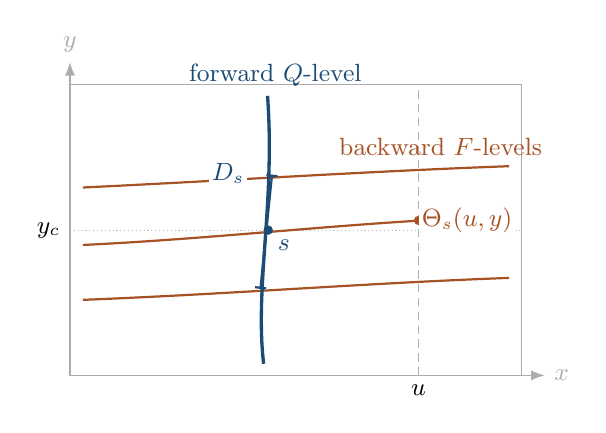
\begin{tikzpicture}[x=0.82cm,y=0.82cm,>=Latex,font=\small]
  \definecolor{leafblue}{RGB}{28,75,118}
  \definecolor{sweeporange}{RGB}{167,82,36}
  \draw[gray!65] (0,0) rectangle (7,4.5);
  \draw[gray!65,->] (0,0) -- (7.35,0) node[right] {$x$};
  \draw[gray!65,->] (0,0) -- (0,4.85) node[above] {$y$};
  \draw[gray!55,densely dotted] (0,2.25) -- (7,2.25);
  \node[left] at (0,2.25) {$y_c$};
  \draw[gray!60,densely dashed] (5.4,0) -- (5.4,4.5);
  \node[below] at (5.4,0) {$u$};
  \draw[sweeporange,thick]
    (0.2,1.17) .. controls (2.5,1.26) and (4.6,1.43) .. (6.8,1.51);
  \draw[sweeporange,thick]
    (0.2,2.02) .. controls (2.5,2.13) and (4.6,2.40) .. (6.8,2.46);
  \draw[sweeporange,thick]
    (0.2,2.91) .. controls (2.5,3.02) and (4.6,3.16) .. (6.8,3.24);
  \draw[leafblue,very thick]
    (3.0,0.18) .. controls (2.86,1.35) and (3.18,2.69) .. (3.06,4.33);
  \fill[leafblue] (3.07,2.25) circle (1.7pt);
  \node[below right,leafblue] at (3.07,2.25) {$s$};
  \draw[leafblue,thick,{Bar[width=4pt]}-{Bar[width=4pt]}]
    (2.95,1.34) -- (3.13,3.11);
  \node[left,leafblue,fill=white,inner sep=1pt] at (2.75,3.13) {$D_s$};
  \fill[sweeporange] (5.4,2.40) circle (1.7pt);
  \node[right,sweeporange,fill=white,inner sep=1pt]
    at (5.4,2.40) {$\Theta_s(u,y)$};
  \node[above,leafblue] at (3.18,4.32) {forward $Q$-level};
  \node[above,sweeporange] at (5.74,3.25) {backward $F$-levels};
\end{tikzpicture}
\caption{Coordinate schematic for the bridge change of variables, not
an orbit plot. A forward level is labelled at $y=y_c$ by $s$; the
eligible slice $D_s$ is swept across the square along transverse
backward levels to the coordinate $(u,\Theta_s(u,y))$.}
\label{bridge:sweep-figure}
\end{figure}


\paragraph{Forward labels and their area.}
Assume first that $H$ is at the forward end and $W$ at the backward
end. Cover the middle-time torus by the finitely many closed squares
of a grid of side $s_0=1/32$ in a fundamental domain. Overlaps on
boundaries have area zero and cause no problem for an upper bound.
Fix one square $I_x\times I_y$ and choose $y_c\in I_y$. All position
functions in this square and its small neighborhood are computed
from the same real lifted recurrence starting at $(x,y)$.

Every forward graph through an eligible point in the square extends
over all of $I_y$, with a margin, since its parameter range has length
$1/2$ and $s_0<1/4$. Label it by its intercept $s$ at $y=y_c$ and
write it as $(X(s,y),y)$. Two such graphs which meet have the same
value of $Q$ and coincide locally because $Q_x\ne0$. They then
coincide on the whole common interval: the coincidence set is both
open, by implicit uniqueness, and closed, by continuity. In
particular distinct labels have disjoint images at every fixed $y$.

Let $E$ be the labels of forward graphs through forward-eligible
points of this square for which $H\geq h$. We use closed eligibility
conditions, including \cref{bridge:row-choice}. They and $H\geq h$
define a compact subset of the closed square. Continuous dependence
of the graph in \cref{bridge:graphs} makes its intercept a continuous
function of the initial point. Thus $E$ is compact. The graph is
uniquely determined by its intercept, so these constructions define
$X$ unambiguously on $E\times I_y$.

For these labels, every point of the graph over $I_y$ has $H>h/2$ by
\cref{bridge:observation-error}. The identity
\[
 Q(X(s,y),y)=Q(s,y_c)
\]
and implicit differentiation give
\begin{equation}
 X_s(s,y)=\frac{Q_x(s,y_c)}{Q_x(X(s,y),y)}.
 \label{bridge:label-jacobian}
\end{equation}
The derivative in \cref{bridge:label-jacobian} is interpreted through
a local smooth extension when $E$ has empty interior; the existence
of that extension is justified below. The distortion assertion of
\cref{bridge:graphs} bounds its absolute value above and below by
positive constants.

The map $(s,y)\mapsto(X(s,y),y)$ on $E\times I_y$ is injective and
has Jacobian comparable to 1. Its image stays in a fixed bounded
lift: the small slope bounds the displacement from the square by an
absolute constant. Projection of this bounded lift to the torus has
bounded multiplicity. Change of variables therefore yields
\begin{equation}
 \abs E\leq C\PP(H>h/2).
 \label{bridge:label-area}
\end{equation}
The factor $\abs{I_y}=s_0$ has been absorbed into the constant.

\paragraph{A transverse sweep for the weight.}
Fix $s\in E$. Let $D_s\subseteq I_y$ consist of the parameters $y$
for which $z(y)=(X(s,y),y)$ lies in the square and is backward-eligible
in the fixed backward endpoint choice. This is a compact set. Carry
each $z(y)$ along its backward graph to first coordinate $u\in I_x$,
and denote the resulting second coordinate by $\Theta_s(u,y)$.
The carry is defined throughout $I_x$, with a margin.

For each fixed $u$, the map $y\mapsto\Theta_s(u,y)$ is injective on
$D_s$. If two carried points agreed, their backward graphs would
coincide throughout $I_x$ by regular-level uniqueness. A single such
graph cannot meet the chosen forward graph in two distinct points:
two intersections would satisfy both
$\abs{\Delta x}\leq a_0\abs{\Delta y}$ and
$\abs{\Delta y}\leq a_0\abs{\Delta x}$, forcing equality of the
points. This proves the asserted injectivity.

The equation defining the carry is
\[
 F(u,\Theta_s(u,y))=F(X(s,y),y).
\]
Differentiation with respect to the starting parameter gives
\begin{equation}
 \partial_y\Theta_s(u,y)
 =\frac{F_y(z(y))+F_x(z(y))X_y(s,y)}
        {F_y(u,\Theta_s(u,y))}.
 \label{bridge:sweep-jacobian}
\end{equation}
The ratio of the two $F_y$ terms is uniformly bounded above and
below along the backward graph. Moreover $\abs{F_x/F_y}\leq a_0$
at its starting point, since $-F_x/F_y$ is its slope, and
$\abs{X_y}\leq a_0$. Hence the absolute value of
\cref{bridge:sweep-jacobian} is uniformly bounded above and below
by positive constants.

The endpoint observation estimate gives, for all $u\in I_x$ and
$y\in D_s$,
\[
 W(X(s,y),y)\leq W(u,\Theta_s(u,y))+\delta_n.
\]
Apply change of variables to the injective map
$(u,y)\mapsto(u,\Theta_s(u,y))$ on $I_x\times D_s$.
Its image lies in a bounded lift. Since $W\geq0$, its integral over
that image is at most a fixed multiple of $\E W$. Using
\cref{bridge:sweep-jacobian} and then dividing by $\abs{I_x}$ gives
\begin{equation}
 \int_{D_s}W(X(s,y),y)\,\dd y
 \leq C\bigl(\E W+M^{-\sigma n}\bigr).
 \label{bridge:conditional-weight}
\end{equation}

\paragraph{Changes of variables on the eligible subsets.}
Here are details ensuring that the preceding changes of variables
do not require the eligible sets to have interior. Consider first
one forward graph with label $s$. It is a compact regular level arc
over $I_y$ and extends with a margin beyond this interval. The
partial derivative $Q_x$ is nonzero on the arc. The implicit
function theorem in finitely many overlapping charts along the arc
therefore continues it smoothly for intercepts in an open
neighborhood of $s$. The continued level is prescribed by
$Q(s',y_c)$ for each nearby intercept $s'$. Uniqueness in the
overlapping charts makes these local continuations consistent.
Every nearby eligible label follows the same continuation, because
its regular graph passes through that intercept. Thus $X$ on
$E\times I_y$ is locally the restriction of a smooth function of
$(s,y)$, and \cref{bridge:label-jacobian} holds at all required
points.

For the transverse sweep, fix $s$ and a point of $D_s$. Its backward
graph is likewise a compact regular arc, with $F_y\ne0$, extending
with margin over $I_x$. The same continuation argument applies to
the smoothly varying starting points $(X(s,y),y)$ on the fixed
forward graph. It gives a local smooth extension of
$\Theta_s(u,y)$ in both variables, agreeing with all nearby
eligible carries by uniqueness. The maps used in both area
comparisons are consequently restrictions of local smooth
diffeomorphisms, with the displayed nonvanishing Jacobians.

A countable cover by such charts can be split into disjoint Borel
pieces. On each piece ordinary change of variables applies to its
measurable subset; the images of the pieces are disjoint because
the full restricted maps are injective. Summing proves the formulas
on the compact eligible domains. This also establishes the
measurability of all integrands and swept regions used above.
No extension of eligibility to a neighborhood is assumed.

\paragraph{Completion of the area comparison.}
Every point of the fixed square satisfying both eligibility
conditions and $H>h$ belongs to a forward graph with label in $E$.
Change variables from $x$ to this label at each $y$, using
\cref{bridge:label-jacobian}. Drop conditions other than square
membership and backward eligibility, which is allowed because the
weight is nonnegative. The desired weighted integral over this
square and this pair of choices is bounded by
\[
 C\int_E\int_{D_s}W(X(s,y),y)\,\dd y\,\dd s.
\]
Combining \cref{bridge:conditional-weight,bridge:label-area} bounds
this by the right side of \cref{bridge:product}.

If $H$ is at the backward end, begin instead with the labels of the
almost horizontal backward graphs and sweep them in the $x$
direction to bound their label measure by $\PP(H>h/2)$. For each
such graph, transport its eligible points along the almost vertical
forward graphs to estimate $W$. The proof just given applies with
$x,y$ and $Q,F$ interchanged: the graph extents, distortion bounds,
small-slope injectivity argument, and local chart construction are
the same. This proves the estimate for the other assignment of the
two observations as well.

Finally sum over the finitely many squares and the at most four
endpoint-coordinate choices. The constants remain uniform. Average
over the usable middle indices as explained after
\cref{bridge:middle-eligibility}. This establishes
\cref{bridge:product} and completes the proof.
\end{proof}

\section{Product distances and measures across scales}
\label{sec:scales}

Suppose, toward a contradiction, that there is a sequence of parameters
$k\to+\infty$ for which the top Lyapunov exponent vanishes almost
everywhere. All limits in this section are taken along this sequence,
passing to subsequences when indicated, except where a fixed-parameter
limit in orbit length is explicitly specified. The structural constants
in \cref{can:theorem,bridge:theorem} are fixed throughout; the bridge
estimate's auxiliary constants may depend on its observation bounds.
Use the growth semimetric $g$ and expected shortfall $e_n$ from
\cref{scale:distance-deficit}; their parameter dependence remains
suppressed. At each parameter in the sequence, the zero-exponent
assumption and bounded convergence give
\begin{equation}\label{scale:long-deficit}
e_n\longrightarrow1\qquad(n\to\infty).
\end{equation}
By contrast, the shortfall at every fixed length tends to zero as the
parameter grows. We will select a dyadic range in which the shortfall
first increases, and sum the loss between each whole interval and its
two halves over that range. This sum telescopes, but its limiting mass
must still be controlled near arrays with one constant growth rate.
The local tests and measures below are designed to retain that mass.

\Needspace{8\baselineskip}
\subsection{Four-point comparison and truncation}

\begin{lemma}[Four-point comparison]\label{scale:fourpoint}
Fix a base index $i$ and write
\[
 D_j=\norm{T_{i,j}},\qquad
 R_{jp}=M^{g(j,p)-g(i,j)-g(i,p)}.
\]
There is an absolute constant $C_0\ge1$ such that, for every orbit,
every sufficiently large parameter, and every choice of integer indices,
\begin{equation}\label{scale:R-fourpoint}
 R_{jp}\le C_0\max\{R_{jl},R_{lp}\}.
\end{equation}
\end{lemma}

\begin{proof}
Choose a most expanded unit input direction $a_j$ for $T_{i,j}$;
if $D_j=1$, any singular direction may be used. Set
\[
 Q_{jp}=\max\{|a_j\wedge a_p|,D_j^{-2},D_p^{-2}\}.
\]
We claim
\begin{equation}\label{scale:R-comparison}
 Q_{jp}\le R_{jp}\le3Q_{jp}.
\end{equation}
To obtain the sine lower bound, use a unit input at the base
perpendicular to $a_p$. Its norm at $p$ is $D_p^{-1}$, whereas its
norm at $j$ is at least $D_j|a_j\wedge a_p|$. The transfer from $p$
to $j$ therefore has norm at least $D_jD_p|a_j\wedge a_p|$.
The inequalities
\[
 \norm{T_{p,j}}\ge D_j/D_p,\qquad
 \norm{T_{p,j}}\ge D_p/D_j
\]
give the other two lower bounds; the second uses equality of the norms
of a determinant-one matrix and its inverse.

For the upper bound, transport a unit vector from $p$ back to the
base. Its components along $a_p$ and $a_p^\perp$ have absolute values
at most $D_p^{-1}$ and $D_p$, respectively. Also
\[
 \norm{T_{i,j}a_p^\perp}
 \le D_j|a_j\wedge a_p|+D_j^{-1}.
\]
It follows that
\[
 R_{jp}\le D_p^{-2}+|a_j\wedge a_p|+D_j^{-2},
\]
proving \cref{scale:R-comparison}. By
\cref{setup:sine-triangle},
$Q_{jp}\le2\max\{Q_{jl},Q_{lp}\}$, so $C_0=6$ is permissible.
\end{proof}

\begin{lemma}[Truncation of a cancellation]\label{scale:truncation}
Fix integers $i$, $n\ge1$, and $1\le s\le n$, and put
\[
 L=i-n,\quad R=i+n,\quad L'=i-s,\quad R'=i+s,
\]
\[
 D=n-\min\{g(i,L),g(i,R)\},\qquad
 \ell=g(i,L)+g(i,R)-g(L,R).
\]
Use the quantities $R_{uv}$ of \cref{scale:fourpoint} with base $i$.
Then
\begin{align}
 g(i,L'),g(i,R')&\ge s-D,
 \label{scale:cut-wings}\\
 R_{L'R'}&\le C_0^2\max\{R_{LR},M^{-2s+2D}\}.
 \label{scale:cut-R}
\end{align}
There is a constant $A$ independent of the parameter and indices such
that the cut cancellation loss satisfies
\begin{equation}\label{scale:cut-loss}
 g(i,L')+g(i,R')-g(L',R')
 \ge\min\{\ell,2s-2D\}-A,
\end{equation}
and consequently
\begin{equation}\label{scale:cut-full}
 g(L',R')\le2s-\min\{\ell,2s-2D\}+A.
\end{equation}
\end{lemma}

\begin{proof}
The triangle inequality and \cref{scale:distance-bound} give
\[
 g(i,L')\ge g(i,L)-g(L,L')\ge(n-D)-(n-s)=s-D,
\]
and similarly on the right. In particular,
\[
 R_{LL'}\le M^{(n-s)-(n-D)-(s-D)}=M^{-2s+2D},
 \qquad R_{RR'}\le M^{-2s+2D}.
\]
Apply \cref{scale:R-fourpoint} twice along the chain $L',L,R,R'$ to
obtain \cref{scale:cut-R}. Taking negative base-$M$ logarithms gives
\cref{scale:cut-loss}, with any fixed upper bound for
$2\log_M C_0$ as $A$. Such a bound is uniform after imposing, for
example, $M\ge2$. Finally, each cut wing has length at most $s$,
which yields \cref{scale:cut-full}.
\end{proof}

\begin{lemma}[Doubling bound]\label{scale:doubling}
For all sufficiently large parameters and every integer $n\ge1$,
\begin{equation}\label{scale:doubling-equation}
 e_n\le e_{2n}\le C e_n+\frac{C}{n},
\end{equation}
with a constant independent of $n$ and the parameter.
\end{lemma}

\begin{proof}
Use the notation of \cref{scale:truncation}. Both $D$ and $\ell$ are
nonnegative, and $\ell\le2n$. Let $\delta>0$ be the fixed constant
in \cref{can:theorem}. Choose a fixed $H$ sufficiently large that
\[
 \ell>H(1+D),\qquad s=\lfloor\ell/2\rfloor
 \quad\Longrightarrow\quad
 s\ge1,\quad 2D+A\le\delta s.
\]
This is possible since $s\ge\ell/2-1$. Also $s\le n$ and
$2s\le\ell$. Thus \cref{scale:cut-wings,scale:cut-full} imply
\[
 \min\{g(i,i-s),g(i,i+s)\}\ge(1-\delta)s,
 \qquad g(i-s,i+s)\le2D+A\le\delta s.
\]
This is the event bounded by \cref{can:theorem}, with spacing $s$.
On the part where this integer $s$ is selected, $\ell<2s+2$.
Writing the constants of that theorem as $C_{\rm can},\gamma>0$,
we obtain
\[
 \E\bigl[\ell\,\one_{\{\ell>H(1+D)\}}\bigr]
 \le C_{\rm can}\sum_{s=1}^{\infty}(2s+2)e^{-\gamma s}
 \le C.
\]
The complementary contribution is at most $H(1+\E D)$, hence
\begin{equation}\label{scale:mean-cancellation}
 \E\ell\le C(1+\E D).
\end{equation}
Stationarity gives
\[
 \E D\le\E[n-g(i,L)]+\E[n-g(i,R)]=2ne_n,
 \qquad e_{2n}=e_n+\frac{\E\ell}{2n}.
\]
These identities and \cref{scale:mean-cancellation} prove the result.
In particular the lower inequality uses only $\ell\ge0$.
\end{proof}

\Needspace{8\baselineskip}
\subsection{Selecting the first growing deficit}

\begin{lemma}[Critical scales]\label{scale:selection}
Along the assumed zero-exponent parameter sequence, there are powers
of two $n_0=n_0(K)$ and $N=N(K)>n_0$, and numbers $\epsilon=e_N$,
such that
\begin{equation}\label{scale:selected-limits}
 n_0\to\infty,\qquad \epsilon\to0,\qquad
 \epsilon n_0\to\infty,
\end{equation}
and, for every fixed integer $m\in\Z$ (once the lengths below are
positive integers),
\begin{equation}\label{scale:selected-boundaries}
 e_{2^m n_0}=o(\epsilon),\qquad
 e_{2^m N}=O_m(\epsilon).
\end{equation}
All scale sums below run over powers of two.
\end{lemma}

\begin{proof}
First, for every fixed integer $a\ge1$, we have $e_a\to0$ as
$K\to\infty$. To see this, fix $0<\zeta<1$. The uniform marginal
law of each $q_i$ implies
\[
 \PP\{|v(q_i)|<M^{1-\zeta}\}\longrightarrow0.
\]
Indeed $v(x)=2+K\cos(2\pi x)$, and the length of the set on which
$|\cos(2\pi x)|\le(M^{1-\zeta}+2)/K$ tends to zero. A union bound
therefore shows that, with probability tending to one, all $a$
coefficients in the product satisfy $|v(q_i)|\ge M^{1-\zeta}$.
Start the linear recurrence with $(u_0,u_{-1})=(1,0)$. On this event,
for $M$ large, induction gives
\[
 |u_{j+1}|\ge(M^{1-\zeta}-1)|u_j|\ge|u_j|
 \quad(0\le j<a).
\]
Consequently $g(0,a)/a\ge\log_M(M^{1-\zeta}-1)$ there.
The deficit always lies in $[0,1]$, so
$\limsup_{K\to\infty}e_a\le\zeta$. Letting $\zeta\downarrow0$
proves the claim.

Choose powers of two $n_0\to\infty$ sufficiently slowly that
$e_{n_0}\to0$, by diagonal selection over the fixed lengths
$1,2,4,\ldots$. Set
\[
 \theta_K=(n_0^{-1}+e_{n_0})^{1/2}.
\]
For all sufficiently large $K$, $e_{n_0}<\theta_K<1$.
By \cref{scale:long-deficit}, there is a first power of two
$N\ge n_0$ for which $e_N>\theta_K$. It satisfies $N>n_0$ and
$e_{N/2}\le\theta_K$. Applying \cref{scale:doubling} once gives
\[
 \theta_K<\epsilon=e_N\le C\theta_K+C/n_0\longrightarrow0.
\]
Also $\epsilon n_0\ge\theta_K n_0\ge\sqrt{n_0}\to\infty$.
For fixed $m\ge0$, iteration of \cref{scale:doubling} yields
\[
 e_{2^m n_0}\le C_m(e_{n_0}+n_0^{-1})
 =C_m\theta_K^2=o(\epsilon),
\]
and
\[
 e_{2^m N}\le C_m(\epsilon+N^{-1})=O_m(\epsilon).
\]
For a fixed negative $m$, the lengths $2^m n_0$ and $2^mN$ are
eventually positive integers. Dyadic monotonicity bounds their
deficits by $e_{n_0}=o(\epsilon)$ and $e_N=\epsilon$, respectively.
This proves every assertion.
\end{proof}

\subsection{A compact space of distance arrays}

The next construction records shortfall increments as measures on
rescaled distance arrays. Its output will be locally finite limits
away from affine arrays, together with a dilation balance; the
discarded affine part requires separate control in the final argument.

Let $\mathcal D=\Z[1/2]$ denote the dyadic rational numbers. Define
$X$ to be the set of symmetric semimetric arrays
$d:\mathcal D\times\mathcal D\to[0,\infty)$ satisfying
\begin{equation}\label{scale:ambient-bound}
 d(s,t)\le|s-t|+2.
\end{equation}
Give $X$ the topology of pointwise convergence. It is a closed subset
of a countable product of compact intervals, and hence is compact
and metrizable. Its compact subset of affine arrays is
\[
 \mathcal A=\{d_w:0\le w\le1\},\qquad d_w(s,t)=w|t-s|.
\]
These are precisely the arrays of this form that belong to $X$:
the bound at arbitrarily large separations forces $w\le1$.
Write $\mathcal U=X\setminus\mathcal A$.

For a positive integer $n$, define the random array
\begin{equation}\label{scale:rescaled-array}
 g_n(s,t)=\frac{g(\lfloor ns\rfloor,\lfloor nt\rfloor)}{n}
 \qquad(s,t\in\mathcal D).
\end{equation}
It belongs to $X$, since its distances are at most
$|s-t|+1/n$. Introduce the finite measures
\begin{equation}\label{scale:prelimit-measures}
 \mu_K=\epsilon^{-1}\sum_{\substack{n_0\le n<N\\n\text{ a power of }2}}
                  \Law(g_n),\qquad
 \nu_K=\epsilon^{-1}\Law(g_N),\qquad
 \xi_K=\epsilon^{-1}\Law(g_{n_0}).
\end{equation}
Their total masses need not remain bounded. We will obtain limits on
$\mathcal U$ by controlling local departures from affinity.

For an interval $I=[s,t]$ with distinct dyadic endpoints, let $I_l,I_r$
be its left and right halves and define continuous functions on $X$ by
\begin{equation}\label{scale:tests}
 h(I)=1-\frac{d(s,t)}{t-s},\qquad
 J(I)=h(I)-\frac{h(I_l)+h(I_r)}{2},\qquad
 V(I)=\bigl(h(I_l)-h(I_r)\bigr)^2.
\end{equation}
The functions $J(I)$ and $V(I)$ are nonnegative on all of $X$.
The first assertion is the triangle inequality. The shortfall $h(I)$
itself need not be nonnegative on all of $X$. It does belong to $[0,1]$
on a sample $g_n$ whenever the endpoints multiplied by $n$ are integers.
For any fixed dyadic interval, this alignment holds at every scale
$n\ge n_0$ occurring here once $K$ is sufficiently large.

\begin{lemma}[Bounds for local tests]\label{scale:local-mass}
Let $I$ have dyadic endpoints and length $p=2^m$, where $m\in\Z$ is
fixed. Then
\begin{equation}\label{scale:sum-test-bound}
 \int\bigl(J(I)+V(I)\bigr)\,\dd\mu_K=O_I(1).
\end{equation}
Uniformly over the individual dyadic scales $n_0\le n\le N$,
\begin{equation}\label{scale:individual-test-bound}
 \epsilon^{-1}\E\bigl[h(I)(g_n)+J(I)(g_n)+V(I)(g_n)\bigr]
 =O_I(1).
\end{equation}
At the initial scale the stronger bound holds:
\begin{equation}\label{scale:initial-test-bound}
 \epsilon^{-1}\E\bigl[h(I)(g_{n_0})+J(I)(g_{n_0})
                         +V(I)(g_{n_0})\bigr]=o(1).
\end{equation}
All three statements concern sufficiently large $K$, so that the
indicated endpoints and half-endpoints align.
\end{lemma}

\begin{proof}
By stationarity,
\[
 \E h(I)(g_n)=e_{pn},\qquad
 \E J(I)(g_n)=e_{pn}-e_{pn/2}.
\]
Summation over consecutive dyadic scales gives the exact identity
\begin{equation}\label{scale:J-telescope}
 \sum_{\substack{n_0\le n<N\\n\text{ a power of }2}}
       \E J(I)(g_n)=e_{pN/2}-e_{pn_0/2}.
\end{equation}
By \cref{scale:selection} and dyadic monotonicity, its nonnegative
right side is $O_I(\epsilon)$.

Put $a=h(I_l)$, $b=h(I_r)$, and $\bar h=(a+b)/2$. At the aligned
sampled arrays, $0\le\bar h\le h(I)\le1$, and therefore
\begin{align*}
 \frac{V(I)}4
 &=\frac{a^2+b^2}{2}-\bar h^2\\
 &\le\frac{a^2+b^2}{2}-h(I)^2+2J(I).
\end{align*}
Write $b_q=\E\bigl[(1-g(0,q)/q)^2\bigr]$ for integer $q\ge1$.
By stationarity and another dyadic telescoping,
\[
 \frac14\sum_n\E V(I)(g_n)
 \le b_{pn_0/2}-b_{pN/2}
      +2\bigl(e_{pN/2}-e_{pn_0/2}\bigr)
 \le b_{pn_0/2}+2e_{pN/2}.
\]
Here and in this display only, the unqualified sum is over the scales
in \cref{scale:J-telescope}. Since $0\le b_q\le e_q$, the last
expression is $O_I(\epsilon)$. This proves
\cref{scale:sum-test-bound}.

At any single aligned scale, $J(I)\le h(I)$ and
$V(I)=(a-b)^2\le a+b$. Hence the expectation in
\cref{scale:individual-test-bound} is at most
$2e_{pn}+2e_{pn/2}$. Dyadic monotonicity bounds these terms by the
corresponding terminal-scale deficits, which are $O_I(\epsilon)$
by \cref{scale:selection}. At $n=n_0$ they are $o(\epsilon)$,
again by that lemma, including its consequence for negative shifts.
\end{proof}

\begin{lemma}[Detection of affinity]\label{scale:affinity-tests}
As $I$ ranges over intervals with dyadic endpoints and power-of-two
length, the common zero set of $J(I)+V(I)$ is exactly $\mathcal A$.
Consequently, every compact subset $F\subset\mathcal U$ admits
finitely many such intervals $I_1,\ldots,I_b$ and a number $c_F>0$
such that
\begin{equation}\label{scale:finite-test-cover}
 \sum_{a=1}^{b}\bigl(J(I_a)+V(I_a)\bigr)\ge c_F
 \quad\hbox{on }F.
\end{equation}
\end{lemma}

\begin{proof}
Every affine array annihilates these tests. Conversely, suppose they
all vanish. For one of the stated intervals $I$, the equalities
$J(I)=V(I)=0$ say that its two halves have the same speed as $I$
and that their distances add to the full distance. Repeating this
argument shows that every edge of every dyadic subdivision of $I$
has distance $w_I$ times its length, with
$w_I=d(s,t)/(t-s)$. The triangle inequality gives the same upper
bound between any two subdivision nodes. Applying the triangle
inequality across the full interval, using those nodes as intermediate
points, gives the reverse bound, and therefore equality. Every dyadic
point of $I$ is a subdivision node at some level. Apply this argument
to $[-2^a,2^a]$ for arbitrarily large integers $a$. The common pair
$0,1$ fixes one speed on all these intervals, so the array is globally
affine. The ambient bound forces that speed to lie in $[0,1]$.

For the last assertion, each point of $F$ has a positive test. The
corresponding open sets cover $F$, and a finite subcover suffices.
Their sum has a positive minimum on the compact set $F$.
\end{proof}

\Needspace{8\baselineskip}
\subsection{Locally finite limits and their symmetries}

The limiting inequality \cref{scale:tree-inequality} is the
zero-hyperbolic Gromov-product condition: after identifying points at
zero semimetric distance, $B_v(s,t)/2$ is the Gromov product based at $v$;
see \cite[Section~2.2, Definition~2.10]{Bestvina1997}.
The determinant-one estimate and the passage to the limiting arrays
are proved here; no real-tree representation theorem is used.

\begin{proposition}[Limits away from affinity]\label{scale:limits}
After passing to a subsequence, the restrictions of $\mu_K$ and
$\nu_K$ to $\mathcal U$ converge vaguely to locally finite
nonnegative Borel measures $\mu$ and $\nu$, respectively. Moreover,
\begin{equation}\label{scale:initial-negligible}
 \xi_K\longrightarrow0\quad\hbox{vaguely on }\mathcal U.
\end{equation}
The measures $\mu$ and $\nu$ are supported on the closed class
$X_0\subset X$ consisting of arrays satisfying $d(s,t)\le|s-t|$
and the inequalities
\begin{equation}\label{scale:tree-inequality}
 B_v(s,t)\ge\min\{B_v(s,p),B_v(p,t)\},\qquad
 B_v(s,t)=d(v,s)+d(v,t)-d(s,t)
\end{equation}
for every $v,s,t,p\in\mathcal D$. Every member of $X_0$ extends
uniquely to a continuous semimetric on $\R$, obeying the same
inequalities at all real arguments. Both limiting measures are
invariant under
\[
 (\tau_r d)(s,t)=d(s+r,t+r)\qquad(r\in\mathcal D).
\]
For every interval $I$ as in \cref{scale:local-mass},
\begin{equation}\label{scale:limiting-test-bound}
 \int(J(I)+V(I))\,\dd\mu<\infty,
 \qquad
 \int(h(I)+J(I)+V(I))\,\dd\nu<\infty.
\end{equation}
In particular,
\begin{equation}\label{scale:terminal-shortfall}
 \int h([0,1])\,\dd\nu\le1.
\end{equation}
\end{proposition}

\begin{proof}
For each compact $F\subset\mathcal U$, combine
\cref{scale:finite-test-cover} with
\cref{scale:sum-test-bound,scale:individual-test-bound} to obtain
uniform bounds on $\mu_K(F)$ and $\nu_K(F)$. Using
\cref{scale:initial-test-bound} instead gives $\xi_K(F)=o(1)$.
The latter proves \cref{scale:initial-negligible}, since a continuous
compactly supported test is bounded and has compact support.

Here is an explicit way to extract the local limits. Fix a compatible
metric on $X$ and let $a(d)=\dist(d,\mathcal A)$. Choose a continuous
nondecreasing function $\chi:[0,\infty)\to[0,1]$ equal to zero on
$[0,1/2]$ and to one on $[1,\infty)$. Set
$\chi_j(d)=\chi(2^j a(d))$. These functions increase to one on
$\mathcal U$, have compact support there, and satisfy
$\chi_{j+1}=1$ on $\supp\chi_j$. The finite measures
$\chi_j\mu_K$ and $\chi_j\nu_K$ have bounded total masses for
each $j$. Weak compactness for finite measures on compact metric
spaces, followed by a diagonal extraction, gives weak limits for
all of them. Their restrictions agree on the open regions where the
corresponding cutoffs are one: this follows by testing against
continuous functions supported in such a region, for which the
prelimit integrals agree. These compatible restrictions define
locally finite measures on $\mathcal U$. Every compactly supported
continuous function is supported where some $\chi_j$ is one, so
these are the asserted vague limits.

For completeness, the support restrictions survive despite the
possibly unbounded total masses. The arrays $g_n$ satisfy
$g_n(s,t)\le|s-t|+1/n$. Taking logarithms in
\cref{scale:R-fourpoint}, then dividing by $n$, shows that their
version of \cref{scale:tree-inequality} has error at most
$(\log_M C_0)/n$. These errors are bounded uniformly by $C/n_0$
at every sampled scale. Any fixed strict violation, by a fixed
positive margin, is thus absent from every sampled array once $K$
is large. Testing on compact subsets of its open violation set
shows that it has zero limiting measure. There are countably many
dyadic arguments and positive rational margins, which proves the
stated support assertion. For an array with $d(s,t)\le|s-t|$,
the semimetric inequality gives
\[
 |d(s,t)-d(s',t')|\le|s-s'|+|t-t'|.
\]
It therefore has a unique jointly continuous extension to real
arguments; all its inequalities extend by continuity.

For fixed $r\in\mathcal D$, each prelimit law is invariant under
$\tau_r$ once $n_0r$ is an integer. Indeed
$\lfloor n(s+r)\rfloor=\lfloor ns\rfloor+nr$, and stationarity
applies simultaneously to the array. The map $\tau_r$ is a
homeomorphism of $X$ preserving $\mathcal A$, so it preserves
compact support in $\mathcal U$. Invariance therefore passes to
the vague limits.

Finally, multiply any nonnegative test $J(I)+V(I)$ by $\chi_j$,
pass to the vague limit, and use
\cref{scale:sum-test-bound}. Monotone convergence as $j\to\infty$
gives the first bound in \cref{scale:limiting-test-bound}. For $\nu$
use \cref{scale:individual-test-bound} in the same way. Although
$h(I)$ is not nonnegative everywhere on $X$, it is nonnegative on
the aligned samples and on the supported limiting class $X_0$;
these facts justify the cutoff bounds and monotone convergence for
that term as well. In the case $I=[0,1]$ the uncut terminal
integral is exactly $e_N/\epsilon=1$, giving
\cref{scale:terminal-shortfall}.
\end{proof}

Define the dilation
\begin{equation}\label{scale:dilation}
 (Sd)(s,t)=\frac{d(2s,2t)}2.
\end{equation}
It is a continuous map from $X$ into $X$ and fixes every affine
array. Its inverse need not map all of $X$ into $X$, but on $X_0$
it is the homeomorphism
\[
 (S^{-1}d)(s,t)=2d(s/2,t/2).
\]
Both maps preserve $X_0\cap\mathcal U$.

\begin{proposition}[Positive dilation decomposition]\label{scale:decomposition}
On $\mathcal U$, with the measures supported on $X_0$ as above,
\begin{equation}\label{scale:measure-balance}
 S_*\mu=\mu+\nu.
\end{equation}
There is a locally finite nonnegative measure $\mu_\infty$, invariant
under $S$ and every dyadic translation, such that
\begin{equation}\label{scale:measure-decomposition}
 \mu=\mu_\infty+\sum_{j=1}^{\infty}(S^{-j})_*\nu,
 \qquad S_*\mu_\infty=\mu_\infty.
\end{equation}
The series is a series of positive measures dominated by $\mu$.
\end{proposition}

\begin{proof}
The floor convention in \cref{scale:rescaled-array} gives the exact
identity $Sg_n=g_{2n}$. Hence, as finite measures on $X$,
\begin{equation}\label{scale:finite-measure-balance}
 S_*\mu_K=\mu_K+\nu_K-\xi_K.
\end{equation}
To pass to the local limits, observe that $S^{-1}(\mathcal A)
=\mathcal A$: multiplication by two permutes the dyadic rationals,
so $Sd=d_w$ implies $d=d_w$. If $F\subset\mathcal U$ is compact,
its preimage under $S$ is closed in compact $X$ and disjoint from
$\mathcal A$, hence compact in $\mathcal U$. Thus $S$ is proper
on $\mathcal U$, and composition with $S$ preserves continuous
compactly supported tests there. Vague convergence and
\cref{scale:initial-negligible} now give
\cref{scale:measure-balance}.

We may henceforth work on $X_0\cap\mathcal U$, where $S$ is
invertible. Applying its inverse to \cref{scale:measure-balance}
and iterating gives, for every $b\ge1$,
\[
 \mu=(S^{-b})_*\mu+\sum_{j=1}^{b}(S^{-j})_*\nu.
\]
The increasing positive partial sums are dominated by $\mu$.
Their limit
$\lambda=\sum_{j\ge1}(S^{-j})_*\nu$ is therefore a locally finite
measure. On relatively compact Borel sets define
$\mu_\infty=\mu-\lambda$. The definitions agree on overlaps and
extend by exhaustion to a locally finite nonnegative measure;
this construction avoids subtracting infinite total masses.
Monotone convergence for the positive series yields
\[
 S_*\lambda=\nu+\lambda.
\]
Subtract this identity from \cref{scale:measure-balance} on
relatively compact sets to obtain $S_*\mu_\infty=\mu_\infty$.

For $r\in\mathcal D$ and $j\ge1$, the identity
\[
 \tau_r S^{-j}=S^{-j}\tau_{r/2^j}
\]
and translation invariance of $\nu$ show that every summand of
$\lambda$ is invariant under $\tau_r$. The same holds for their
sum and, by local subtraction from the translation-invariant
measure $\mu$, for $\mu_\infty$. This proves all assertions.
\end{proof}

\section{Support restrictions and the geometry of limiting distances}
\label{shape:section}

Throughout this section we retain the sequence of parameters, scales, and
measures constructed in \cref{scale:selection,scale:limits}.  In particular,
all limiting arrays belong to $X_0$, and all measures are considered on
$\mathcal U=X\setminus\mathcal A$.  As before, $\mathcal D$ denotes the
dyadic rationals.  The constants $\delta$ and $c_b$ are those fixed in
\cref{can:theorem,bridge:theorem}; neither depends on the scales or the
parameter sequence.

For $d\in X_0$, let $P_d$ be the set of times having no open neighborhood
on which $d(x,y)=w|x-y|$ for some constant $w$, and let $Q_d$ be the set
of times having no open neighborhood on which $d(x,y)=|x-y|$.
These sets are closed, and $P_d\subset Q_d$.  Here and below a property of
the distance on an interval concerns every pair of points in that interval.

\begin{proposition}[Support exclusions]\label{shape:exclusions}
There is a measurable set of full measure for $\mu$, $\nu$, and
$\mu_\infty$ on which the following statements hold for every real choice
of their arguments.
\begin{enumerate}
\item There do not exist $r\in\R$ and $t>0$ such that
\begin{equation}\label{shape:forbidden-triple}
 d(r-t,r)>(1-\delta)t,\qquad
 d(r,r+t)>(1-\delta)t,\qquad
 d(r-t,r+t)<\delta t.
\end{equation}
\item If $s\in P_d$ and $t\in Q_d$, then
\begin{equation}\label{shape:slow-pair}
 d(s,t)\le c_b|t-s|.
\end{equation}
\end{enumerate}
The same statements hold almost everywhere for every positive measure
appearing in the decomposition of \cref{scale:decomposition}.
\end{proposition}

\begin{proof}
First fix $r,t\in\mathcal D$, $t>0$.  For all sufficiently large $K$,
$nr$ and $nt$ are integers at every scale $n\ge n_0$ in our sums.
The event \cref{shape:forbidden-triple} for $g_n$ is contained in the
cancellation event of \cref{can:theorem}, at center $nr$ and spacing
$nt$.  Consequently its $\mu_K$-mass is at most
\[
 \frac{C}{\epsilon}\sum_{n_0\le n<N}^{\rm dyadic}
 e^{-\gamma tn}
 \le \frac{C_t}{\epsilon}e^{-\gamma t n_0}\longrightarrow0.
\]
The last conclusion follows from $\epsilon n_0\to\infty$ in
\cref{scale:selection}.  The event is open in $X$.  To pass to a locally
finite limit, test its indicator from below by nonnegative continuous
functions with compact support in $\mathcal U$.  This shows that its
$\mu$-mass is zero.  Taking the countable union over $r,t\in\mathcal D$
and then using continuity of $d$ excludes every real triple: strict
inequalities at a real center and spacing persist at nearby dyadic ones.

We record explicitly the weighted consequence of the bridge estimate
needed for the second exclusion.  Fix a bridge $[u,v]$ with dyadic
endpoints and length $r=v-u>0$.  Fix a power-of-two interval $I$ in the
allowed window about one endpoint and another such interval $I'$ in the
allowed window about the other endpoint.  The two endpoints can be
interchanged.  Put
\[
 W=J(I)+V(I),\qquad H=h(I'),
\]
and fix a threshold $\eta>0$.  These are fixed bounded Lipschitz
functions of finitely many shortfalls, and $W\ge0$.  All their endpoints
align with the integer times at every scale in the sum once $K$ is large.
By \cref{scale:individual-test-bound} and Markov's inequality,
\[
 \sup_{n_0\le n<N}^{\rm dyadic}\PP(H(g_n)>\eta/2)
 \le C_{I',\eta}\epsilon.
\]
Applying \cref{bridge:theorem} at the integer bridge length $rn$, summing,
and using \cref{scale:local-mass}, we obtain
\begin{align}
 &\int \one_{\{d(u,v)>c_b r,\ H>\eta\}}W\,\dd\mu_K
 \nonumber\\
 &\qquad\le C\epsilon\left[
       \int W\,\dd\mu_K+
       \frac1\epsilon\sum_{n_0\le n<N}^{\rm dyadic}
                              M^{-\sigma rn}\right]
 \longrightarrow0.\label{shape:weighted-bridge}
\end{align}
Indeed the first bracketed term is bounded, and the second tends to zero:
the exponential sum is at most $2M^{-\sigma r n_0}$ for all sufficiently
large $K$, whereas $1/\epsilon=o(n_0)$.  All constants and thresholds in
this application are fixed before $K$ tends to infinity.  The lower bounds
on $M$ and on bridge length in \cref{bridge:theorem} therefore hold
eventually; no uniformity over varying test intervals is being assumed.

Suppose now that \cref{shape:slow-pair} fails for some $s\in P_d$,
$t\in Q_d$.  Necessarily $s\ne t$.  Choose nearby distinct dyadic bridge
endpoints so that their distance still exceeds $c_b$ times their temporal
separation.  The endpoints can be chosen close enough to $s,t$ that
sufficiently small neighborhoods of these two times fit in the respective
bridge windows.  Some test $J(I)+V(I)$ with power-of-two length and dyadic
endpoints contained in the first neighborhood is positive.  To see this,
choose such an interval containing $s$ in its interior.  If the tests for
it and all its dyadic subdivisions vanished, successive subdivision,
equal half speeds, and equality in the triangle inequality would make
$d$ affine on that interval, contrary to $s\in P_d$.  In the second
neighborhood there is similarly a power-of-two interval $I'$ with
$h(I')>0$.  In fact exact unit distance between the endpoints of any
interval forces exact unit distance on every subinterval, by the triangle
inequality and $d(x,y)\le|x-y|$; hence an interval containing $t$ in its
interior cannot have zero shortfall.

Choose a positive rational $\eta<h(I')$.  The resulting strict bridge
and shortfall conditions define an open set.  By
\cref{shape:weighted-bridge}, its $W\mu$-mass is zero, using compactly
supported continuous tests in $\mathcal U$ as above.  Its part with $W>0$
therefore has zero $\mu$-mass.  There are only countably many choices of
the bridge, the two tests, their orientation, and the rational threshold.
Every violation is covered by one of these choices, proving
\cref{shape:slow-pair} simultaneously for all real $s,t$.

Both properties are invariant under every translation and positive
dilation of time, including the corresponding division of distances by
the dilation factor.  The measure inequality
$(S^{-1})_*\nu\le\mu$ from \cref{scale:decomposition} consequently transfers
them to $\nu$.  All the other component measures are dominated by $\mu$,
so they inherit them as well.  This also provides a measurable full-measure
set: the exceptional sets were covered by countably many measurable
strict tests before extension to real arguments.
\end{proof}

The local-to-global propagation below uses this zero-hyperbolic
Gromov-product framework \cite[Section~2.2]{Bestvina1997}, with an
explicit argument on the semimetric arrays rather than an invocation
of a theorem about geodesic real trees.

\begin{proposition}[Shape classification]\label{shape:classification}
Every nonaffine array in $X_0$ satisfying \cref{shape:exclusions} has one
of the following forms:
\begin{enumerate}
\item every secant has speed at most $c_b$;
\item there is one exterior ray of exact unit speed, and the complementary
closed half-line has all secant speeds at most $c_b$;
\item there are two exterior rays of exact unit speed, separated by a
closed interval $[a,b]$ of positive length, and every secant contained in
$[a,b]$ has speed at most $c_b$.
\end{enumerate}
The second possibility includes either orientation.  These descriptions
do not assert additivity of distances across the slow part.
The three temporal configurations are illustrated in \cref{shape:figure}.
\end{proposition}

\begin{proof}
We first show that a connected component $U$ of $\R\setminus P_d$ is
affine with a single speed throughout.  Its local speeds agree on
overlapping neighborhoods, and hence are a common $w\in[0,1]$ by
connectedness.  A compact subinterval of $U$ has a sufficiently fine
partition $x_0<\cdots<x_m$ such that each consecutive triple lies in a
local affine neighborhood.  When $w=0$, the triangle inequality
immediately gives $d(x_0,x_m)=0$.  When $w>0$, propagate additivity
inductively.  Suppose it holds from $x_0$ through $x_j$, and use the
four-point inequality of \cref{scale:tree-inequality} at base $v=x_j$ in its
limiting form
\begin{equation}\label{shape:tree-inequality}
 B_v(x,z)\ge\min\{B_v(x,y),B_v(y,z)\},\qquad
 B_v(x,z)=d(v,x)+d(v,z)-d(x,z).
\end{equation}
The inductive additivity gives
$B_v(x_0,x_{j-1})=2d(x_{j-1},x_j)>0$, whereas local additivity gives
$B_v(x_{j-1},x_{j+1})=0$.  Apply
\cref{shape:tree-inequality} to the latter pair with intermediate point
$x_0$.  Nonnegativity of $B_v$ forces $B_v(x_0,x_{j+1})=0$, exactly the
next additivity statement.  The first two steps are already locally
affine.  Thus $d(x_0,x_m)=w(x_m-x_0)$, and varying the compact subinterval
proves the claim.  In particular $P_d\ne\varnothing$ for a nonaffine
array.

Suppose a component $U$ has speed $w>c_b$.  It has at least one finite
endpoint $s\in P_d$, since $U=\R$ would imply affinity.  If $w<1$, every
interior point $t\in U$ belongs to $Q_d$.  Continuity at the endpoint gives
$d(s,t)=w|t-s|$, contradicting \cref{shape:slow-pair}.  Therefore $w=1$.
Such a component cannot have two finite endpoints: they would both belong
to $P_d\subset Q_d$, and their unit mutual speed would again contradict
\cref{shape:slow-pair}.  Hence every component of speed greater than
$c_b$ is an exterior unit ray; there are at most two.

Let $I$ be the closed complement of these rays.  It is the whole line, a
closed half-line, or a closed bounded interval.  For $x<y$ in $I$, if
$[x,y]\cap P_d$ is empty, the two points lie in a component of speed at
most $c_b$.  Otherwise let $p$ and $q$ be the first and last points of
$[x,y]\cap P_d$.  The portions from $x$ to $p$ and from $q$ to $y$ have
speed at most $c_b$, by the component claim and continuity.  The middle
portion satisfies the same bound by \cref{shape:slow-pair}, because
$p,q\in P_d\subset Q_d$.  The triangle inequality gives
$d(x,y)\le c_b(y-x)$.  The only case not yet settled is a bounded slow
interval of length zero; \cref{shape:crossloss} below excludes it.
\end{proof}

\begin{lemma}[Loss across two rays]\label{shape:crossloss}
Suppose there are two exterior unit rays with slow interval $[a,b]$,
and put $L=b-a$.  Then $L>0$, and, with the fixed constant
\begin{equation}\label{shape:cross-constant}
 C_*=2+\frac6\delta,
\end{equation}
every $z\in\R$ and $t>0$ satisfy
\begin{equation}\label{shape:cross-bound}
 0\le 1-\frac{d(z,z+t)}t\le\frac{C_*L}{t}.
\end{equation}
The shortfall is zero whenever the interval is wholly in either closed
unit ray.
\end{lemma}

\begin{proof}
For the moment permit $L=0$.  Write
$x_u=a-u$, $y_v=b+v$, where $u,v\ge0$, and put $D=d(a,b)\le L$.
Set
\[
 s=\frac{u+v-D-d(x_u,y_v)}2.
\]
If $s\le0$, the absolute shortfall of $[x_u,y_v]$ is at most
$L+D\le2L$.  Suppose $s>0$.  The reverse triangle inequalities imply
$d(x_u,y_v)\ge u-D-v$ and $d(x_u,y_v)\ge v-D-u$, so that
$s\le\min\{u,v\}$.  At base $a$ the unit rays and triangle inequalities
give
\begin{align*}
 B_a(x_u,x_s)&=2s,\\
 B_a(x_u,y_v)&\ge u+(v-D)-d(x_u,y_v)=2s,\\
 B_a(y_v,y_s)&\ge(v-D)+(s-D)-(v-s)=2s-2D.
\end{align*}
Twice applying \cref{shape:tree-inequality} yields
$B_a(x_s,y_s)\ge2s-2D$.  As $d(a,x_s)=s$ and
$d(a,y_s)\le D+s$, it follows that
\begin{equation}\label{shape:matched-ray-distance}
 d(x_s,y_s)\le3D\le3L.
\end{equation}

Use the temporal midpoint $m=(a+b)/2$ and spacing $t_*=s+L/2$.
Its two wing distances obey
\[
 d(x_s,m),\ d(m,y_s)\ge s-L/2.
\]
If $L>0$ and $s>3L/\delta$, these bounds are strictly greater than
$(1-\delta)t_*$ and \cref{shape:matched-ray-distance} is strictly less
than $\delta t_*$.  This is the forbidden triple of
\cref{shape:forbidden-triple}.  If $L=0$, every $s>0$ produces that same
strict contradiction.  Thus always $s\le3L/\delta$.  A full crossing
interval has absolute shortfall
\[
 (u+L+v)-d(x_u,y_v)=L+D+2s\le C_*L.
\]
An interval meeting only part of the slow interval has absolute
shortfall at most twice the length of that part.  For example, if
$x<a\le y\le b$, then
$d(x,y)\ge(a-x)-d(a,y)\ge(a-x)-(y-a)$, giving loss at most $2(y-a)$.
The other orientation is identical.  An interval inside $[a,b]$ has loss
at most its length, hence at most $L$, and intervals in the unit rays
have zero loss.  This proves \cref{shape:cross-bound} in every case.
If $L=0$, these conclusions would give exact unit distance between every
pair of times, an affine array.  Nonaffinity therefore forces $L>0$.
\end{proof}

\begin{figure}[tb]
\centering
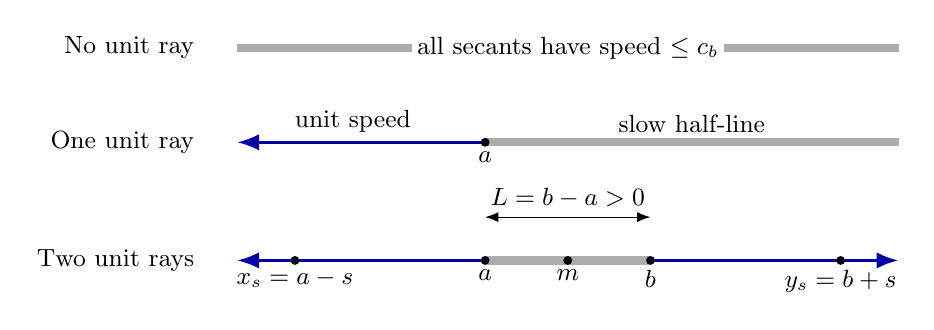
\begin{tikzpicture}[x=1.05cm,y=1cm,>=Latex,font=\small]
  \node[anchor=east] at (-4.4,2.7) {No unit ray};
  \draw[gray!65,line width=3pt] (-4,2.7)--(4,2.7);
  \node[fill=white,inner sep=2pt] at (0,2.7) {all secants have speed $\le c_b$};
  \node[anchor=east] at (-4.4,1.5) {One unit ray};
  \draw[blue!65!black,line width=1.1pt,->] (-1,1.5)--(-4,1.5);
  \draw[gray!65,line width=3pt] (-1,1.5)--(4,1.5);
  \fill (-1,1.5) circle (1.6pt);
  \node[above] at (-2.6,1.5) {unit speed};
  \node[above] at (1.5,1.5) {slow half-line};
  \node[below] at (-1,1.5) {$a$};
  \node[anchor=east] at (-4.4,0) {Two unit rays};
  \draw[blue!65!black,line width=1.1pt,->] (-1,0)--(-4,0);
  \draw[gray!65,line width=3pt] (-1,0)--(1,0);
  \draw[blue!65!black,line width=1.1pt,->] (1,0)--(4,0);
  \draw[<->] (-1,.55)--(1,.55) node[midway,above] {$L=b-a>0$};
  \foreach \x in {-3.3,-1,0,1,3.3}{\fill (\x,0) circle (1.6pt);}
  \node[below] at (-3.3,0) {$x_s=a-s$};
  \node[below] at (-1,0) {$a$};
  \node[below] at (0,0) {$m$};
  \node[below] at (1,0) {$b$};
  \node[below] at (3.3,0) {$y_s=b+s$};
\end{tikzpicture}
\caption{The possible temporal regions in \cref{shape:classification};
the one-ray picture may also be reflected.  A slow region need not be
affine.  In the bottom picture, excessive loss between the exterior rays
would produce the symmetric forbidden triple $(x_s,m,y_s)$ used in
\cref{shape:crossloss}.  The diagram describes time regions, not an
embedding of the semimetric.}
\label{shape:figure}
\end{figure}

\FloatBarrier
\section{A capped deficit and the final balance}
\label{end:section}

The cap will compare the slow interval of a limiting shape at fine and
coarse scales. It must equal one on uniformly slow secants. For a
two-ray shape, \cref{shape:cross-bound} makes the shortfall of a long
crossing interval small; a sufficiently small slope of the cap near
zero will make its averaged coarse contribution smaller than the
fine-scale occupancy of the slow interval. This is an integrated
comparison, not a pointwise sign assertion for the observable below.

Choose a fixed $\alpha>0$ so small that $10C_*\alpha<1$.  Choose a smooth
nondecreasing function $\Phi:[0,1]\to[0,1]$ such that
\begin{equation}\label{end:cap}
 \Phi(u)=\alpha u\ \text{near }0,\qquad
 \Phi(u)=1\quad(1-c_b\le u\le1).
\end{equation}
For completeness, one can choose a nonnegative smooth derivative equal
to $\alpha$ near zero, zero near $1-c_b$, and with integral one on
$[0,1-c_b]$, by adding a nonnegative bump supported strictly between the
two endpoint neighborhoods.  Integrating and continuing constantly gives
\cref{end:cap}.  Positivity near zero and compactness give constants
$0<c_\Phi\le C_\Phi<\infty$ with
\begin{equation}\label{end:linear-bounds}
 c_\Phi u\le\Phi(u)\le C_\Phi u\qquad(0\le u\le1).
\end{equation}
Extend $\Phi$ smoothly to the real line, keeping it linear immediately
to the left of zero.  The extension only defines continuous tests on
$X$; the arrays used below have the relevant shortfalls in $[0,1]$.

Write $h_t(z)=1-d(z,z+t)/t$, and abbreviate $J=J([0,2])$ and
$V=V([0,2])$.  Define
\begin{equation}\label{end:G-definition}
 G(d)=\Phi(h_2(0))-\tfrac12\Phi(h_1(0))-\tfrac12\Phi(h_1(1)).
\end{equation}
If $a=h_1(0)$, $b=h_1(1)$, and $\bar a=(a+b)/2$, then
$h_2(0)=\bar a+J$ and $V=(a-b)^2$.  The mean value theorem followed by
the second-order symmetric Taylor bound yields
\begin{equation}\label{end:G-bound}
 |G|\le\|\Phi'\|J+\frac18\|\Phi''\|V\le C(J+V),
\end{equation}
where the derivative norms can be taken on the compact argument range
of these three tests on $X$.  In particular $G$ is $\mu$-integrable by
\cref{scale:limiting-test-bound}.

At the terminal scale, $\int h_1(0)\,\dd\nu_K=1$.  After a subsequence,
\cref{end:linear-bounds} therefore gives a limit
\begin{equation}\label{end:H-definition}
H_\Phi=\lim_K\int\Phi(h_1(0))\,\dd\nu_K,
 \qquad c_\Phi\le H_\Phi\le C_\Phi.
\end{equation}

There are three steps to the contradiction. First, dyadic telescoping
will give $\int G\,\dd\mu=H_\Phi$, with no loss of weighted mass to
$\mathcal A$. Then the positive decomposition of
\cref{scale:decomposition} separates this integral into a terminal
contribution and the contribution of the invariant remainder. We prove
that the former is strictly less than $H_\Phi$ and the latter is
nonpositive. The cap's two prescribed behaviors enter precisely in
these comparisons.

\begin{proposition}[Exact limiting balance]\label{end:balance}
With the preceding choices,
\begin{equation}\label{end:balance-equation}
 \int G\,\dd\mu=H_\Phi>0.
\end{equation}
\end{proposition}

\begin{proof}
Stationarity makes the two half-interval terms in
\cref{end:G-definition} have equal expectation.  Since
$h_2(0;g_n)=h_1(0;g_{2n})$, summing over the dyadic scales gives exactly
\[
 \int G\,\dd\mu_K
 =\int\Phi(h_1(0))\,\dd\nu_K
  -\frac1\epsilon\E\Phi(h_1(0;g_{n_0})).
\]
The final term tends to zero by
\cref{scale:initial-test-bound,end:linear-bounds}.  Thus these integrals
converge to $H_\Phi$.  We must show that this mass does not escape to
$\mathcal A$ under vague convergence.

The measures $J\mu_K$ and $V\mu_K$ have uniformly bounded total mass on
the compact space $X$, and the signed measures $G\mu_K$ have uniformly
bounded total variation by \cref{end:G-bound}.  Take simultaneous weak
limits
\[
 J\mu_K\longrightarrow\lambda_J,\qquad
 V\mu_K\longrightarrow\lambda_V,\qquad
 G\mu_K\longrightarrow\eta.
\]
On $\mathcal U$ they agree with $J\mu$, $V\mu$, and $G\mu$ respectively:
multiply any compactly supported continuous test there by the indicated
continuous weight.  We show that $\eta|_{\mathcal A}=0$ by treating all
three ranges of affine speeds.  Write $d_w(s,t)=w|s-t|$.

\paragraph{Speeds $0\le w\le c_b$.}
Both $\Phi'$ and $\Phi''$ vanish at every shortfall $1-w$ in this compact
speed range, including its boundary $w=c_b$.  For each $\rho>0$ there is
an open neighborhood $U_\rho$ of
$\{d_w:0\le w\le c_b\}$ on which the Taylor argument for
\cref{end:G-bound} gives
\[
 |G|\le\rho(J+V).
\]
Indeed all arguments between the three relevant shortfalls are then
uniformly close to $[1-c_b,1]$, where both derivatives vanish.
For a continuous test supported in $U_\rho$, pass this domination to
the weak limits.  It implies
$|\eta||_{U_\rho}\le\rho(\lambda_J+\lambda_V)|_{U_\rho}$.
The latter positive measure is finite on $X$.  Letting $\rho$ decrease
to zero shows that $\eta$ has zero restriction to this compact set of
affine arrays.

\paragraph{Speeds $c_b<w<1$.}
Choose a fixed positive dyadic $R$ so large that the endpoint windows of
the bridge $[0,R]$ contain $[0,2]$ and $[R,R+1]$ respectively; for
example require $\kappa R>2$.  Put $W=J+V$ and
$H=h([R,R+1])$.  For each positive rational $\eta_0$, the open set
\[
 U_{\eta_0}=\{d:d(0,R)>c_bR,\ h([R,R+1])>\eta_0\}
\]
has $W\mu_K$-mass tending to zero by
\cref{shape:weighted-bridge}.  The open-set inequality for weak
convergence of positive measures gives
$(\lambda_J+\lambda_V)(U_{\eta_0})=0$.  Each $d_w$ in the current
speed range belongs to such a set by taking $0<\eta_0<1-w$.
This countable cover and \cref{end:G-bound} show that $\eta$ vanishes
on all intermediate affine speeds.  Notice that the threshold is fixed
separately for each test; no threshold uniform as $w\uparrow1$ is needed.

\paragraph{The speed $w=1$.}
Near $d_1$, all three arguments in \cref{end:G-definition} are in the
linear part of $\Phi$, so $G=\alpha J$.  It remains to prove
$\lambda_J(\{d_1\})=0$.  Fix an inverse power of two $q\in(0,1)$.
For the product over $[0,2n]$, with center $n$, put
\[
 D=n-\min\{g(0,n),g(n,2n)\},\qquad
 \ell=g(0,n)+g(n,2n)-g(0,2n)=2nJ(g_n).
\]
The quantities $D/n$ and $\ell/n$ are continuous tests of $g_n$,
both zero at $d_1$.  Thus the condition
$2q-2D/n>\ell/n$ defines an open neighborhood $U_q$ of $d_1$.
Eventually $s=qn$ is an integer at every scale in the sum.
On $U_q$, the truncation estimate of \cref{scale:truncation} gives,
with its fixed additive constant $A$,
\[
 \ell\le\ell_{\rm cut}+A,
 \qquad
 J\le qJ([1-q,1+q])+\frac{A}{2n}.
\]
The shorter-interval test telescopes exactly, by stationarity:
\[
 \int J([1-q,1+q])\,\dd\mu_K
 =\frac{e_{qN}-e_{qn_0}}\epsilon\le1,
\]
where dyadic monotonicity gives $e_{qN}\le e_N=\epsilon$.
Also $\epsilon^{-1}\sum_n n^{-1}=O((\epsilon n_0)^{-1})=o(1)$.
Since $J\ge0$,
\[
 \int_{U_q}J\,\dd\mu_K\le q+o(1).
\]
The open-set inequality now gives $\lambda_J(U_q)\le q$, so
$\lambda_J(\{d_1\})\le q$.  First take the fixed weak limit and then
let $q$ decrease through inverse powers of two to obtain zero.  The
local identity $G=\alpha J$ transfers this conclusion to $\eta$.

These cases cover $\mathcal A$.  Weak convergence on compact $X$
preserves the total mass of the signed measures, so
$\eta(X)=H_\Phi$.  As $\eta|_{\mathcal A}=0$ and
$\eta|_{\mathcal U}=G\mu$, this is \cref{end:balance-equation}.
\end{proof}

\subsection{The terminal measure and its backward dilates}

The decomposition in \cref{scale:decomposition}, together with
\cref{end:G-bound}, gives an absolutely convergent identity
\begin{equation}\label{end:integrated-decomposition}
 \int G\,\dd\mu
 =\int G\,\dd\mu_\infty
  +\sum_{j=1}^{\infty}\int G(S^{-j}d)\,\dd\nu(d).
\end{equation}
More precisely, the sum of the integrals of $|G(S^{-j}d)|$ is at most
$\int|G|\,\dd\mu$, so all the subsequent rearrangements of these
component integrals are justified.

\begin{lemma}[Strict bound for the terminal contribution]
\label{end:terminal}
The series in \cref{end:integrated-decomposition} satisfies
\begin{equation}\label{end:terminal-strict}
 \sum_{j=1}^{\infty}\int G(S^{-j}d)\,\dd\nu(d)<H_\Phi.
\end{equation}
\end{lemma}

\begin{proof}
Nonnegative compact cutoffs exhausting $\mathcal U$, the terminal
prelimit identities, and monotone convergence imply
\begin{equation}\label{end:terminal-bounds}
 \int h_1(0)\,\dd\nu\le1,
 \qquad \int\Phi(h_1(0))\,\dd\nu\le H_\Phi.
\end{equation}
For each integer $m\ge0$, subdivision and the triangle inequality give
\[
 h_1(0)\ge2^{-m}\sum_{r=0}^{2^m-1}h_{2^{-m}}(r2^{-m}).
\]
Dyadic translation invariance of $\nu$ therefore implies
$\int h_{2^{-m}}(0)\,\dd\nu\le1$.  The same shortfalls inserted into
$\Phi$ have finite integrals, bounded by $C_\Phi$.

Set $A_m=\int\Phi(h_{2^{-m}}(0))\,\dd\nu$.  Translation invariance
at the shift $2^{-j}$ gives
\[
 \int G(S^{-j}d)\,\dd\nu=A_{j-1}-A_j.
\]
Absolute convergence of the series implies convergence of $A_m$.
Fatou's lemma yields
\begin{align}
 \sum_{j=1}^{\infty}\int G(S^{-j}d)\,\dd\nu
 &\le A_0-
    \int\liminf_{m\to\infty}\Phi(h_{2^{-m}}(0))\,\dd\nu
 \nonumber\\
 &\le H_\Phi-
    \int\liminf_{m\to\infty}\Phi(h_{2^{-m}}(0))\,\dd\nu.
 \label{end:terminal-fatou}
\end{align}
If $\nu=0$, the series is zero and \cref{end:H-definition} proves the
strict conclusion.  Otherwise every shape in its full-measure support
has a slow interval with nonempty interior by
\cref{shape:classification,shape:crossloss}.  There is a dyadic $z$ in
that interior.  For all sufficiently large $m$, the interval
$[z,z+2^{-m}]$ is slow, so
$\Phi(h_{2^{-m}}(z))=1$ by \cref{end:cap}.

The measurable sets
\[
 E_z=\{d:\Phi(h_{2^{-m}}(z))=1\text{ for every sufficiently large }m\},
 \qquad z\in\mathcal D,
\]
cover this full-measure support.  At least one has positive $\nu$-measure,
and translation invariance gives $\nu(E_0)=\nu(E_z)>0$.
Consequently the subtracted integral in \cref{end:terminal-fatou} is
positive.  It is finite by Fatou's lemma and the bound $A_m\le C_\Phi$.
This proves \cref{end:terminal-strict} in all cases.
\end{proof}

\subsection{The translation- and dilation-invariant remainder}

We next give the measurable and local-finiteness details needed to
integrate over shapes.  A dyadic interval whose endpoint distance equals
its length has exact unit speed throughout, by the triangle inequality
and the Lipschitz bound.  Thus the local unit-speed set is the union of
the interiors of those countably many intervals.  More directly, define
extended-real endpoint functions on $X_0$ by
\begin{align}
 a(d)&=\sup\{r\in\mathcal D:
       d(p,q)=q-p\text{ for all }p,q\in\mathcal D, p<q<r\},
 \label{end:left-endpoint}\\
 b(d)&=\inf\{r\in\mathcal D:
       d(p,q)=q-p\text{ for all }p,q\in\mathcal D, r<p<q\}.
 \label{end:right-endpoint}
\end{align}
Use $\sup\varnothing=-\infty$ and $\inf\varnothing=+\infty$.
Each ray condition is a countable intersection of closed secant
conditions, so $a,b$ are measurable.  On our nonaffine shapes a finite
$a$ is exactly the right endpoint of the exterior left unit ray, and a
finite $b$ is exactly the left endpoint of the exterior right unit ray.
They obey, for $r\in\mathcal D$,
\begin{equation}\label{end:endpoint-covariance}
 a(\tau_r d)=a(d)-r,\quad b(\tau_r d)=b(d)-r,
 \qquad a(Sd)=a(d)/2,\quad b(Sd)=b(d)/2.
\end{equation}
Thus the three shape classes and the length $L=b-a$ on the two-ray
class are measurable and transform as asserted.

\begin{lemma}[Nonpositive invariant contribution]\label{end:remainder}
The invariant remainder satisfies
\begin{equation}\label{end:remainder-bound}
 \int G\,\dd\mu_\infty\le0.
\end{equation}
\end{lemma}

\begin{proof}
On an entirely slow shape, each shortfall in
\cref{end:G-definition} is at least $1-c_b$, so all three capped values
equal one and $G=0$.

Consider next shapes with exactly one unit ray.  First take the
orientation with a left unit ray and finite interface $a$.
For a bounded interval $[A,B]$ of possible interface locations, choose
one fixed dyadic secant strictly to the left of $A$ and a second strictly
to the right of $B$.  Their speed ratios on every such shape are
respectively $1$ and at most $c_b$.  The arrays with these two prescribed
closed conditions form a compact subset of $X_0$ disjoint from
$\mathcal A$: an affine array would have the same speed on both secants.
Local finiteness of $\mu_\infty$ on $\mathcal U$ therefore implies finite
mass for interfaces in $[A,B]$.

Push the restriction of $\mu_\infty$ to this shape class forward by $a$,
obtaining a measure $\lambda$ on $\R$ finite on bounded intervals.
Its invariances, from \cref{end:endpoint-covariance}, give
\[
 \lambda([0,1))=\lambda([0,2))
 =\lambda([0,1))+\lambda([1,2))=2\lambda([0,1)).
\]
The first equality uses $S$-invariance; the last uses translation by
one.  Finiteness forces $\lambda([0,1))=0$, and integer translates
covering $\R$ show that this entire shape class has zero mass.  The same
argument with left and right reversed treats the other one-ray class.
Half-open intervals make the argument valid without any advance
assumption about endpoint atoms.

It remains to consider the two-ray class.  Restrict to the length band
\[
 \mu_*:=\mu_\infty\big|_{\{\text{two rays},\ 1\le L<2\}}.
\]
This measure is invariant under dyadic translations.  Its left endpoint
has finite intensity on bounded intervals, as follows explicitly.
Partition any bounded range of possible $a$ into finitely many bins
$[k/4,(k+1)/4]$.  In each bin the fixed secant
$[(k+1)/4,(k+2)/4]$ lies in $[a,b]$, since $L\ge1$, and hence has ratio
at most $c_b$.  A fixed dyadic secant to the left of the whole bounded
range has ratio one.  The two conditions again put each bin's arrays
inside a compact subset of $\mathcal U$.  A finite union gives the
claimed finite intensity.  The right endpoint also has finite intensity
on bounded intervals because $1\le b-a<2$ bounds $a$ whenever it bounds
$b$.

Neither endpoint intensity has an atom.  If the mass at some point were
positive, dyadic translation invariance would give the same positive
mass to infinitely many distinct points in a bounded interval,
contradicting local finiteness.  Define the finite number
\[
 I_0=\mu_*\{0\le a<1\}.
\]
Every integer interval of length one has this same endpoint mass.

For $j\in\Z$, let $B_j$ be the two-ray band
$2^j\le L<2^{j+1}$.  Since $S$ divides lengths by two and preserves
$\mu_\infty$,
\[
 \mu_\infty|_{B_j}=(S^{-j})_*\mu_*.
\]
The bands are disjoint and cover the two-ray class.  Integrability of
$|G|$ permits reindexing $j$ to $-j$, yielding
\begin{equation}\label{end:band-series}
 \int_{\rm two\ rays}G\,\dd\mu_\infty
 =\sum_{j\in\Z}\int G(S^j d)\,\dd\mu_*(d),
 \qquad
 \sum_{j\in\Z}\int|G(S^j d)|\,\dd\mu_*<\infty.
\end{equation}

Put $F_j=\int\Phi(h_{2^j}(0))\,\dd\mu_*$.  These quantities are
finite.  Indeed \cref{shape:crossloss} makes the integrand zero unless
$[0,2^j]$ meets $[a,b]$, which requires $-2\le a\le2^j$; the endpoint
intensity on this bounded interval is finite.  Translation invariance
at the dyadic shift $2^j$ gives
\begin{equation}\label{end:F-difference}
 \int G(S^j d)\,\dd\mu_*=F_{j+1}-F_j.
\end{equation}
The absolute convergence in \cref{end:band-series} implies that $F_j$
has finite limits both as $j\to-\infty$ and as $j\to+\infty$.

For the fine-scale limit, use the dominating integrable function
$\one_{\{-2\le a\le1\}}$ for $j\le0$.  Off the null sets
$\{a=0\}$ and $\{b=0\}$, if $a<0<b$, then $[0,2^j]$ is contained
in the slow interval for all sufficiently negative $j$, and the capped
shortfall equals one.  If zero lies outside the slow interval, the
small interval is eventually in a unit ray and its shortfall is zero.
Dominated convergence therefore gives
\begin{equation}\label{end:fine-limit}
 F_{\rm fine}:=\lim_{j\to-\infty}F_j
 =\mu_*\{a<0<b\}\ge\mu_*\{-1\le a<0\}=I_0.
\end{equation}
The inequality uses $L\ge1$; possible equality endpoints have zero mass.

For the coarse-scale limit, \cref{shape:cross-bound} gives
$0\le h_t(0)\le2C_*/t$ throughout this band.  Once $t$ is sufficiently
large, all these shortfalls lie in the linear region of \cref{end:cap},
uniformly in the shape.  Hence
\[
 \int\Phi(h_t(0))\,\dd\mu_*
 \le \frac{2\alpha C_*}{t}\,
                  \mu_*\{-2\le a\le t\}.
\]
For the large dyadic integers $t=2^j$, atomlessness and integer
translation invariance make the last mass $(t+2)I_0$ (the weaker bound
$(t+3)I_0$ would also suffice).  Thus
\begin{equation}\label{end:coarse-limit}
 F_{\rm coarse}:=\lim_{j\to+\infty}F_j
 \le2\alpha C_*I_0.
\end{equation}
Summing \cref{end:F-difference} and applying
\cref{end:fine-limit,end:coarse-limit} now proves
\[
 \int_{\rm two\ rays}G\,\dd\mu_\infty
 =F_{\rm coarse}-F_{\rm fine}
 \le-(1-2\alpha C_*)I_0\le0.
\]
This argument also covers $I_0=0$; in that case integer translates of
$\{0\le a<1\}$ show that $\mu_*=0$.  Together with the entirely slow
and one-ray cases, this establishes \cref{end:remainder-bound}.
\end{proof}

\begin{theorem}[Contradiction and eventual positive entropy]
\label{end:contradiction}
There is no sequence $k\to+\infty$ along which the largest Lyapunov
exponent of $f_k$ is zero almost everywhere.  Consequently
\cref{main:entropy} holds.
\end{theorem}

\begin{proof}
Under the supposed zero-exponent sequence, all the preceding measures
and identities were constructed.  Combining
\cref{end:integrated-decomposition,end:terminal-strict,end:remainder-bound}
gives
\[
 \int G\,\dd\mu<H_\Phi,
\]
contradicting the exact balance \cref{end:balance-equation}.

For every parameter, the top Lyapunov exponent exists almost everywhere
and is nonnegative, since the derivative cocycle has determinant one.
If positivity on a set of positive area failed at arbitrarily large
positive parameters, the exponent would therefore be zero almost
everywhere at each member of a sequence tending to $+\infty$, which has
just been excluded.  There is consequently a finite $k_0$ such that,
for every $k>k_0$, the top exponent is positive on a set of positive
normalized area.  Increasing the threshold gives the same statement
for every $k\ge k_0$.  The entropy formula \cref{main:pesin} gives
$h_m(f_k)>0$ for every such $k$.  In particular the measurable parameter
interval $[k_0+1,k_0+2]$ has positive one-dimensional Lebesgue measure
and satisfies the required assertion.
\end{proof}

\begin{thebibliography}{99}
\addcontentsline{toc}{section}{References}

\bibitem{BergerCarrasco2014}
P.~Berger and P.~D.~Carrasco,
\emph{Non-uniformly hyperbolic diffeomorphisms derived from the standard map},
Communications in Mathematical Physics \textbf{329} (2014), no.~1, 239--262.
\href{https://doi.org/10.1007/s00220-014-1932-1}
{doi:10.1007/s00220-014-1932-1}.

\bibitem{BergerTuraev2019}
P.~Berger and D.~Turaev,
\emph{On Herman's positive entropy conjecture},
Advances in Mathematics \textbf{349} (2019), 1234--1288.
\href{https://doi.org/10.1016/j.aim.2019.04.002}
{doi:10.1016/j.aim.2019.04.002}.

\bibitem{Bestvina1997}
M.~Bestvina,
\emph{Real trees in topology, geometry, and group theory},
arXiv:math/9712210v1 (1997).
\href{https://arxiv.org/abs/math/9712210v1}{arXiv:math/9712210v1}.

\bibitem{BloorLuzzatto2009}
K.~Bloor and S.~Luzzatto,
\emph{Some remarks on the geometry of the standard map},
International Journal of Bifurcation and Chaos \textbf{19} (2009),
no.~7, 2213--2232.
\href{https://doi.org/10.1142/S0218127409024025}
{doi:10.1142/S0218127409024025}.

\bibitem{Blumenthal2021}
A.~Blumenthal,
\emph{Statistical properties for compositions of standard maps with increasing coefficient},
Ergodic Theory and Dynamical Systems \textbf{41} (2021), no.~4, 981--1024.
\href{https://doi.org/10.1017/etds.2019.115}{doi:10.1017/etds.2019.115}.

\bibitem{BlumenthalXueYoung2017}
A.~Blumenthal, J.~Xue, and L.-S.~Young,
\emph{Lyapunov exponents for random perturbations of some area-preserving
maps including the standard map},
Annals of Mathematics \textbf{185} (2017), no.~1, 285--310.
\href{https://doi.org/10.4007/annals.2017.185.1.5}
{doi:10.4007/annals.2017.185.1.5}.

\bibitem{Chirikov1979}
B.~V.~Chirikov,
\emph{A universal instability of many-dimensional oscillator systems},
Physics Reports \textbf{52} (1979), no.~5, 263--379.
\href{https://doi.org/10.1016/0370-1573(79)90023-1}
{doi:10.1016/0370-1573(79)90023-1}.

\bibitem{Duarte1994}
P.~Duarte,
\emph{Plenty of elliptic islands for the standard family of area preserving maps},
Annales de l'Institut Henri Poincar\'e. Analyse non lin\'eaire
\textbf{11} (1994), no.~4, 359--409.
\href{https://www.numdam.org/item/AIHPC_1994__11_4_359_0/}
{Official article record}.

\bibitem{Gorodetski2012}
A.~Gorodetski,
\emph{On stochastic sea of the standard map},
Communications in Mathematical Physics \textbf{309} (2012), no.~1, 155--192.
\href{https://doi.org/10.1007/s00220-011-1365-z}
{doi:10.1007/s00220-011-1365-z}.

\bibitem{HollandLuzzatto2006}
M.~Holland and S.~Luzzatto,
\emph{Stable manifolds under very weak hyperbolicity conditions},
Journal of Differential Equations \textbf{221} (2006), no.~2, 444--469.
\href{https://doi.org/10.1016/j.jde.2005.07.013}{doi:10.1016/j.jde.2005.07.013}.

\bibitem{KatokBurns1994}
A.~Katok, in collaboration with K.~Burns,
\emph{Infinitesimal Lyapunov functions, invariant cone families and
stochastic properties of smooth dynamical systems},
Ergodic Theory and Dynamical Systems \textbf{14} (1994), 757--785.
\href{https://doi.org/10.1017/S0143385700008142}
{doi:10.1017/S0143385700008142}.

\bibitem{Mane1981}
R.~Ma\~n\'e,
\emph{A proof of Pesin's formula},
Ergodic Theory and Dynamical Systems \textbf{1} (1981), no.~1, 95--102.
\href{https://doi.org/10.1017/S0143385700001188}
{doi:10.1017/S0143385700001188}.

\bibitem{Mane1983Errata}
R.~Ma\~n\'e,
\emph{Errata to A proof of Pesin's formula},
Ergodic Theory and Dynamical Systems \textbf{3} (1983), no.~1, 159--160.
\href{https://doi.org/10.1017/S0143385700001863}
{doi:10.1017/S0143385700001863}.

\bibitem{Obata2021}
D.~Obata,
\emph{Uniqueness of the measure of maximal entropy for the standard map},
Commentarii Mathematici Helvetici \textbf{96} (2021), no.~1, 79--111.
\href{https://doi.org/10.4171/CMH/508}{doi:10.4171/CMH/508}.

\bibitem{Oliveira2024}
F.~Oliveira,
\emph{Positive topological entropy for the Standard Map},
arXiv:2404.02209v2 (2024).
\href{https://arxiv.org/abs/2404.02209}{arXiv:2404.02209}.

\bibitem{Oseledets1968}
V.~I.~Oseledets,
\emph{A multiplicative ergodic theorem.
Lyapunov characteristic numbers for dynamical systems},
Transactions of the Moscow Mathematical Society \textbf{19} (1968), 197--231.
\href{https://www.mathnet.ru/eng/mmo214}{Official bibliographic record}.

\bibitem{Pesin1977}
Ya.~B.~Pesin,
\emph{Characteristic Lyapunov exponents and smooth ergodic theory},
Russian Mathematical Surveys \textbf{32} (1977), no.~4, 55--114.
\href{https://doi.org/10.1070/RM1977v032n04ABEH001639}
{doi:10.1070/RM1977v032n04ABEH001639}.

\end{thebibliography}

\end{document}
